%-----------------------Homework------------------------------------
%-------------------Arman Shokrollahi---------------------------------
%---------------------Coding Theory-------------------------------

\documentclass[a4 paper]{article}
% Set target color model to RGB
\usepackage[inner=1.5cm,outer=1.5cm,top=2.5cm,bottom=2.5cm]{geometry}
\usepackage{setspace}
\usepackage[rgb]{xcolor}
\usepackage{pythonhighlight}
\usepackage{verbatim}
\usepackage{amsgen,amsmath,amstext,amsbsy,amsopn,tikz,amssymb,tkz-linknodes}
\usepackage{fancyhdr}
\usepackage[colorlinks=true, urlcolor=blue,  linkcolor=blue, citecolor=blue]{hyperref}
\usepackage[colorinlistoftodos]{todonotes}
\usepackage{rotating}
%\usetikzlibrary{through,backgrounds}
\hypersetup{%
pdfauthor={Arman Shokrollahi},%
pdftitle={Homework},%
pdfkeywords={Tikz,latex,bootstrap,uncertaintes},%
pdfcreator={PDFLaTeX},%
pdfproducer={PDFLaTeX},%
}
%\usetikzlibrary{shadows}
\usepackage[francais]{babel}
\usepackage{booktabs}
\newcommand{\ra}[1]{\renewcommand{\arraystretch}{#1}}

      \newtheorem{thm}{Theorem}[section]
      \newtheorem{prop}[thm]{Proposition}
      \newtheorem{lem}[thm]{Lemma}
      \newtheorem{cor}[thm]{Corollary}
      \newtheorem{defn}[thm]{Definition}
      \newtheorem{rem}[thm]{Remark}
      \numberwithin{equation}{section}

\newcommand{\homework}[6]{
   \pagestyle{myheadings}
   \thispagestyle{plain}
   \newpage
   \setcounter{page}{1}
   \noindent
   \begin{center}
   \framebox{
      \vbox{\vspace{2mm}
    \hbox to 6.28in { {\bf JWST Project \hfill} }
       \vspace{6mm}
       \hbox to 6.28in { {\Large \hfill #1 (#2)  \hfill} }
       \vspace{6mm}
       \hbox to 6.28in { {\it Instructor: #3 \hfill Student: #5} }
       %\hbox to 6.28in { {\it TA: #4  \hfill #6}}
      \vspace{2mm}}
   }
   \end{center}
   \markboth{#5 -- #1}{#5 -- #1}
   \vspace*{4mm}
}

\newcommand{\bbF}{\mathbb{F}}
\newcommand{\bbX}{\mathbb{X}}
\newcommand{\bI}{\mathbf{I}}
\newcommand{\bX}{\mathbf{X}}
\newcommand{\bY}{\mathbf{Y}}
\newcommand{\bepsilon}{\boldsymbol{\epsilon}}
\newcommand{\balpha}{\boldsymbol{\alpha}}
\newcommand{\bbeta}{\boldsymbol{\beta}}
\newcommand{\0}{\mathbf{0}}

\begin{document}
\homework{Meeting Notes \#1}{due 02/15/23 }{McCleary}{}{Eddie Berman}{}
{\begin{tikzpicture}[outline/.style={draw=#1,thick,fill=#1!50}]
\node [outline=red] at (0,1) {\bf Agenda};
\end{tikzpicture}}
\begin{enumerate}
    \item First results from PSF
    \item Share resources on Ill-conditioned Matrices
    \item Ask about upcoming application materials, share progress todate
    \item Lingering questions
    \item Still to-do, wrapper for Piffy

\end{enumerate}

\noindent {\fbox{\it PSF Results}}\\ 
\section{First results from PSF}
\section*{Control Group}
\begin{python}
# How large should the postage stamp cutouts of the stars be?
    stamp_size: 30

model:
    # This model uses a grid of pixels to model the surface brightness distribution.
    type: PixelGrid
    scale: 0.034      # NIRCam ative pixel scale
    size: 26          # Model is 24 x 24 in these pixels
\end{python}\\


\begin{document}

\begin{figure}
  \begin{subfigure}{\linewidth}
  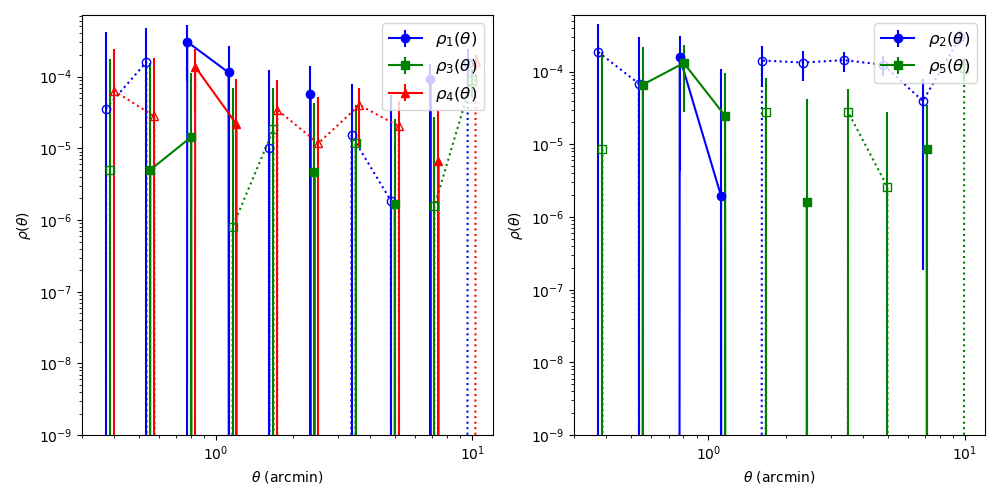
\includegraphics[width=.3\linewidth]{150wControl/piff_rho.png}\hfill
  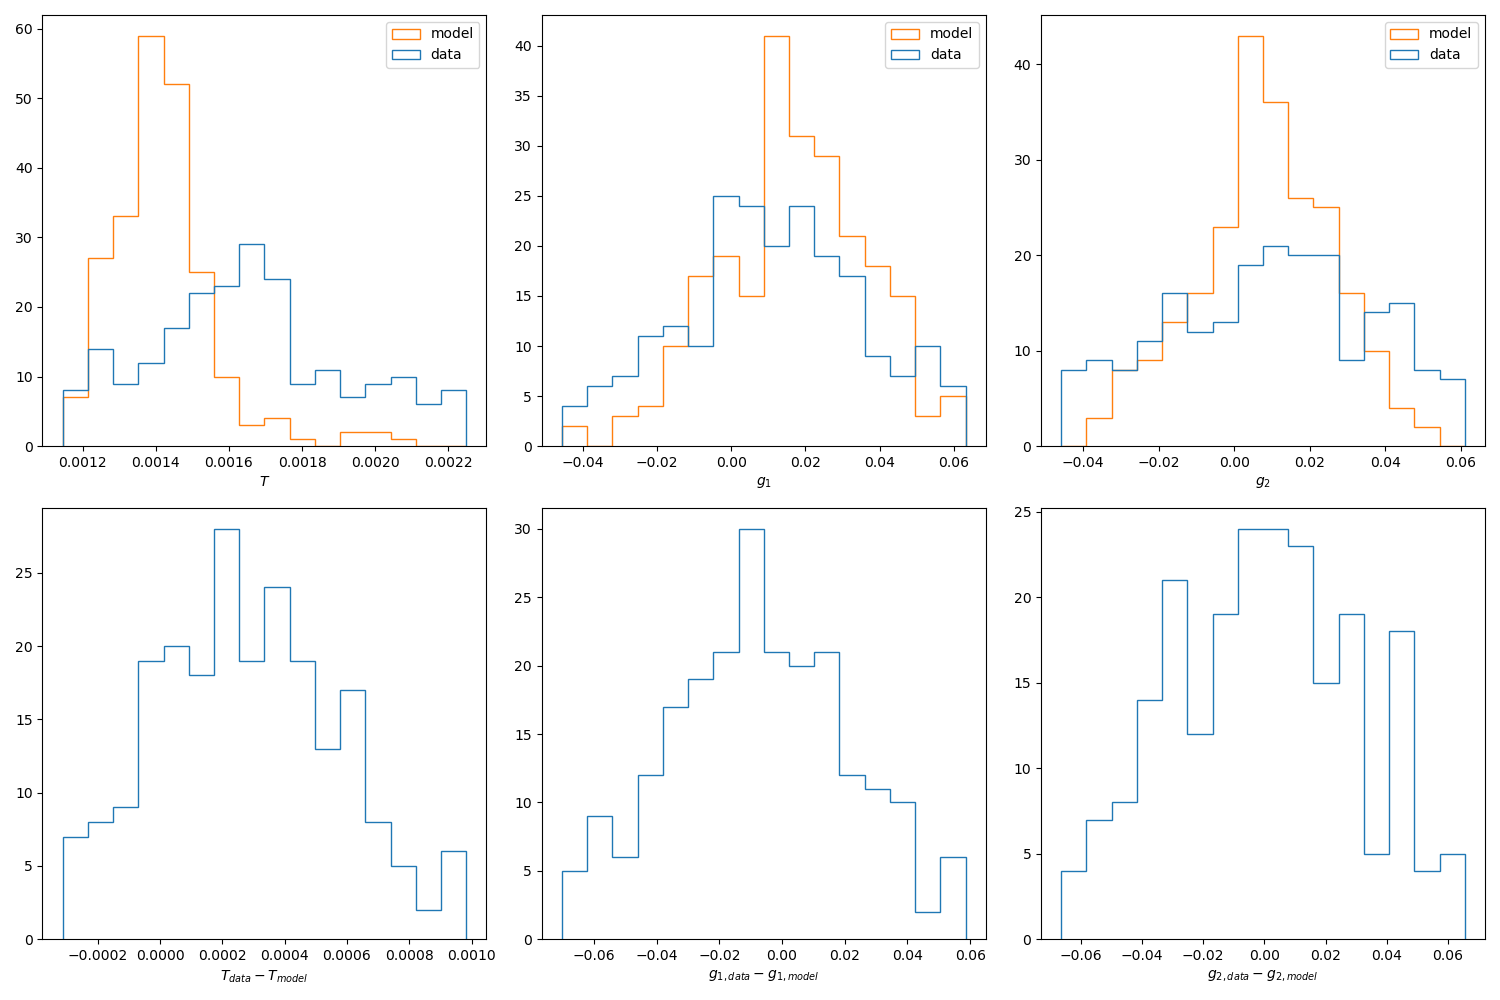
\includegraphics[width=.3\linewidth]{150wControl/piff_shapes.png}\hfill
  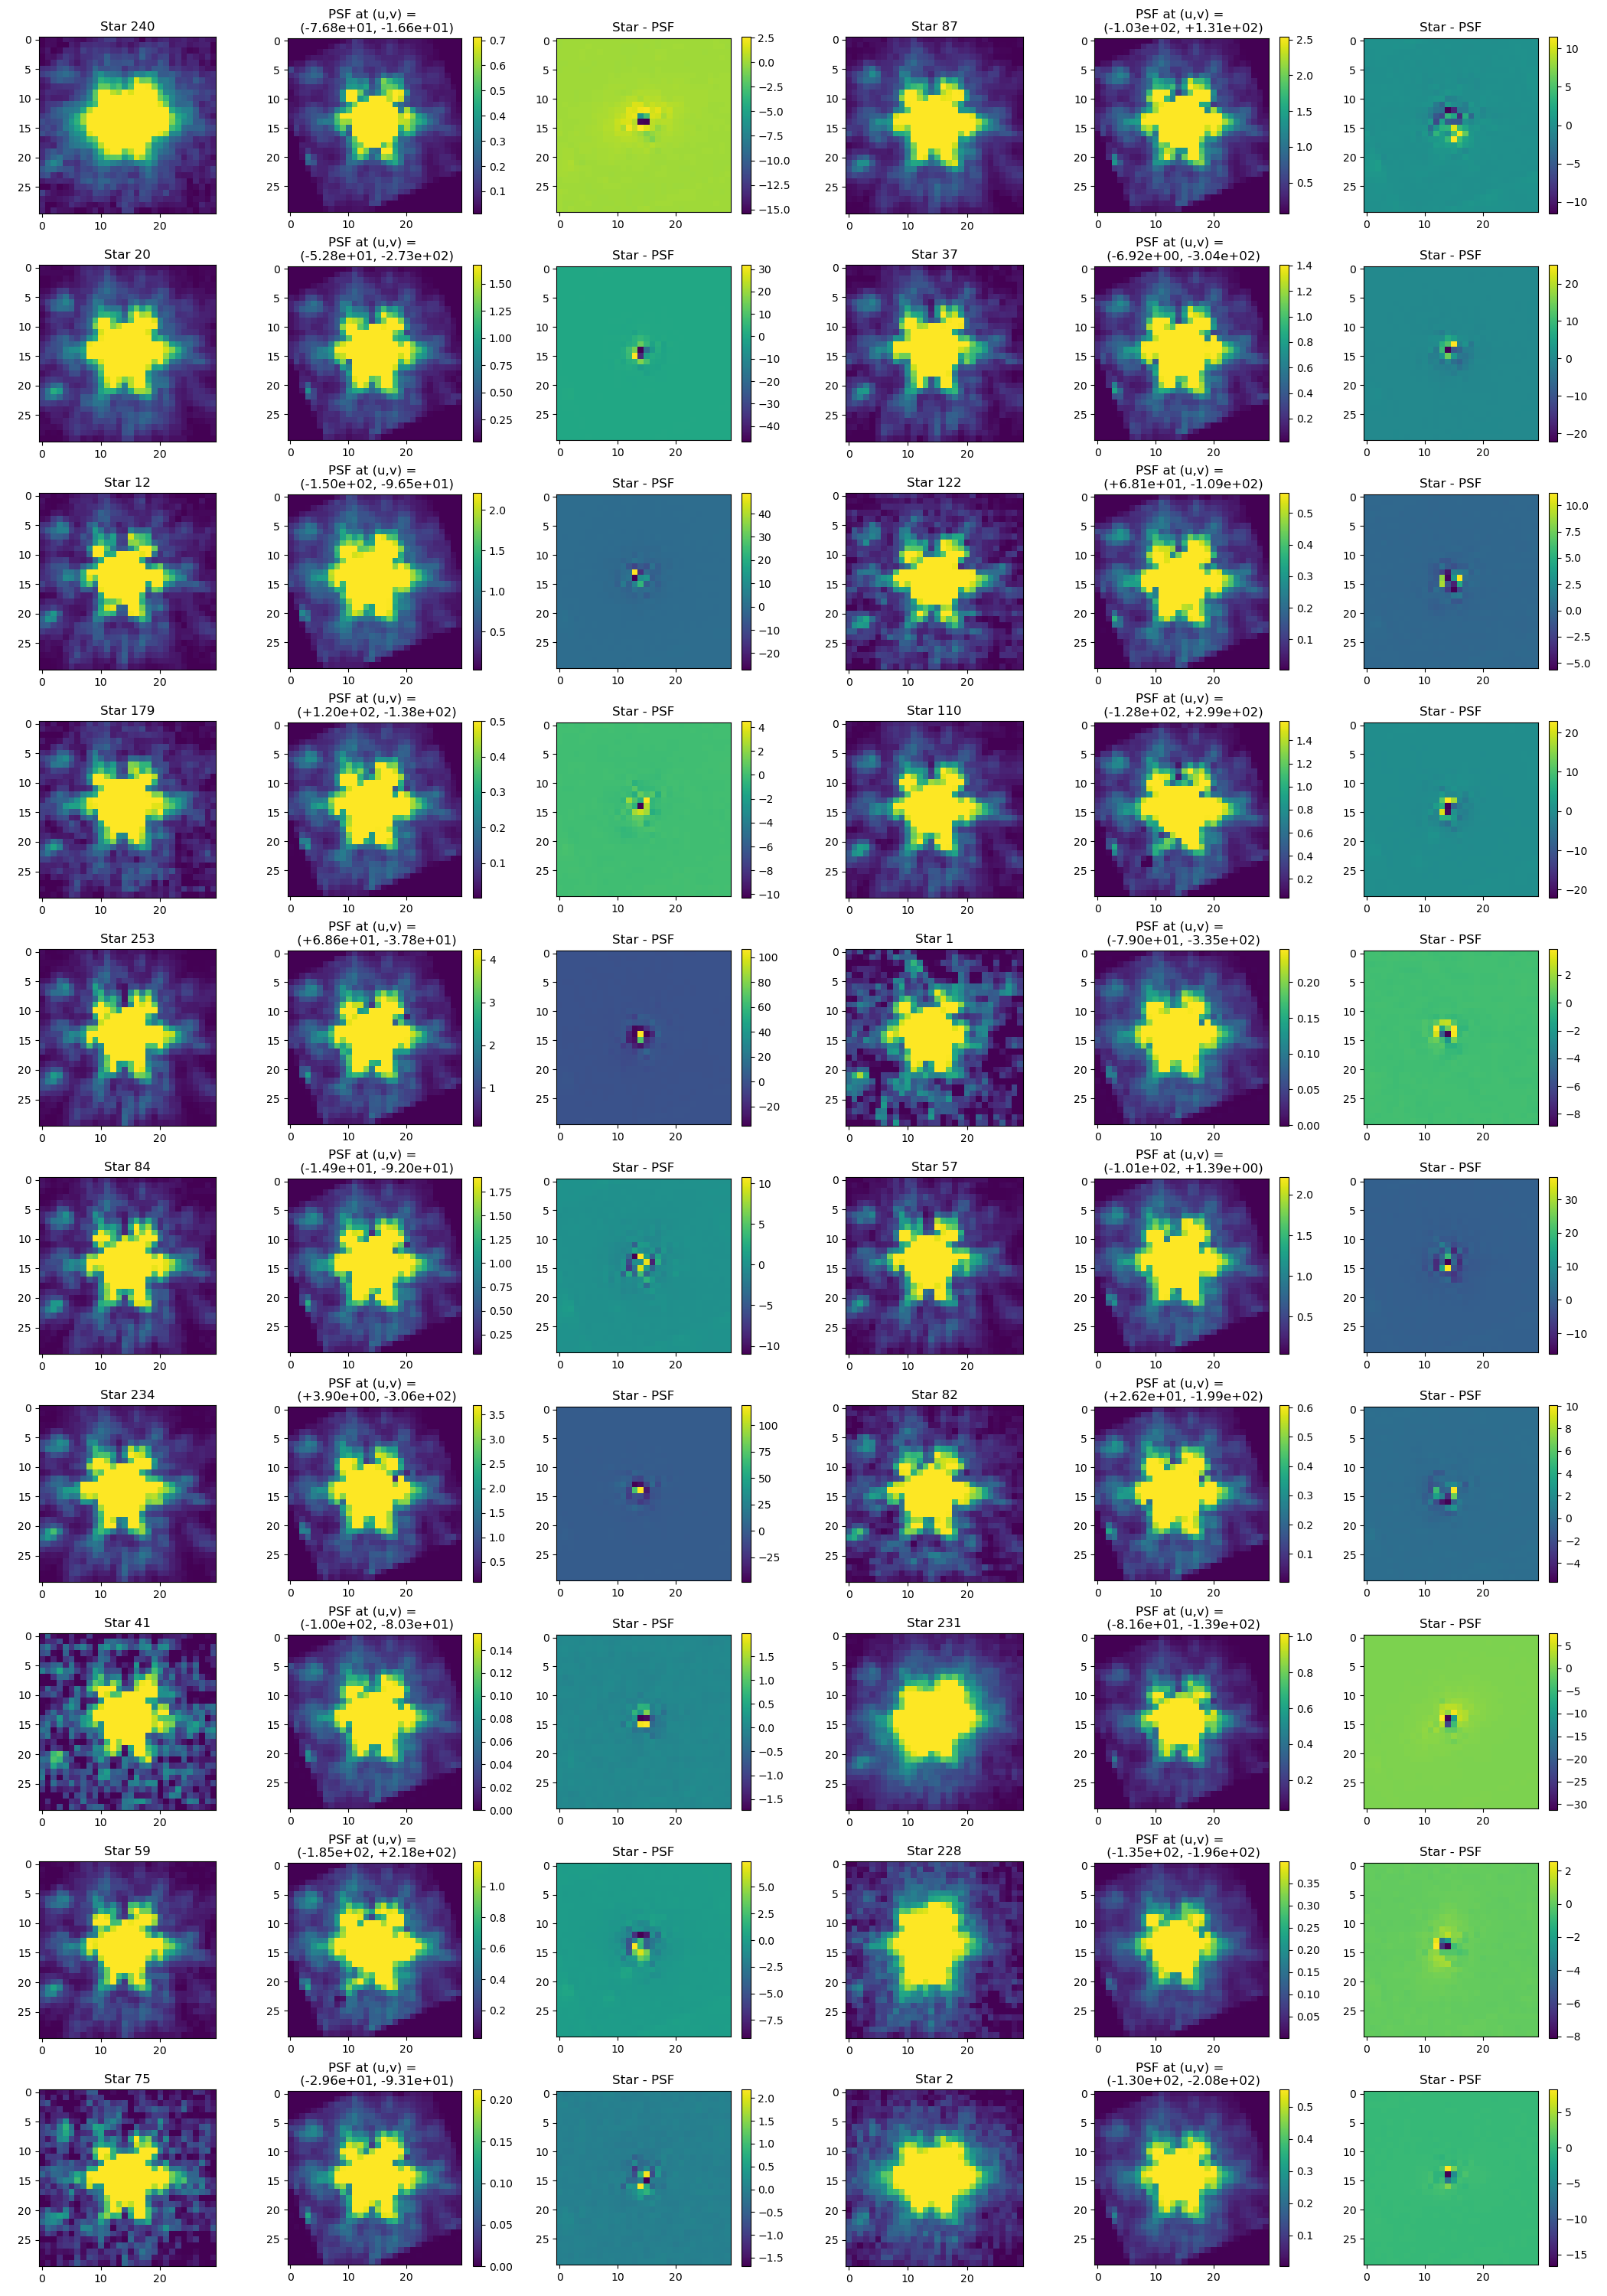
\includegraphics[width=.3\linewidth]{150wControl/piff_stars.png}
  \end{subfigure}\par\medskip
  \begin{subfigure}{\linewidth}
  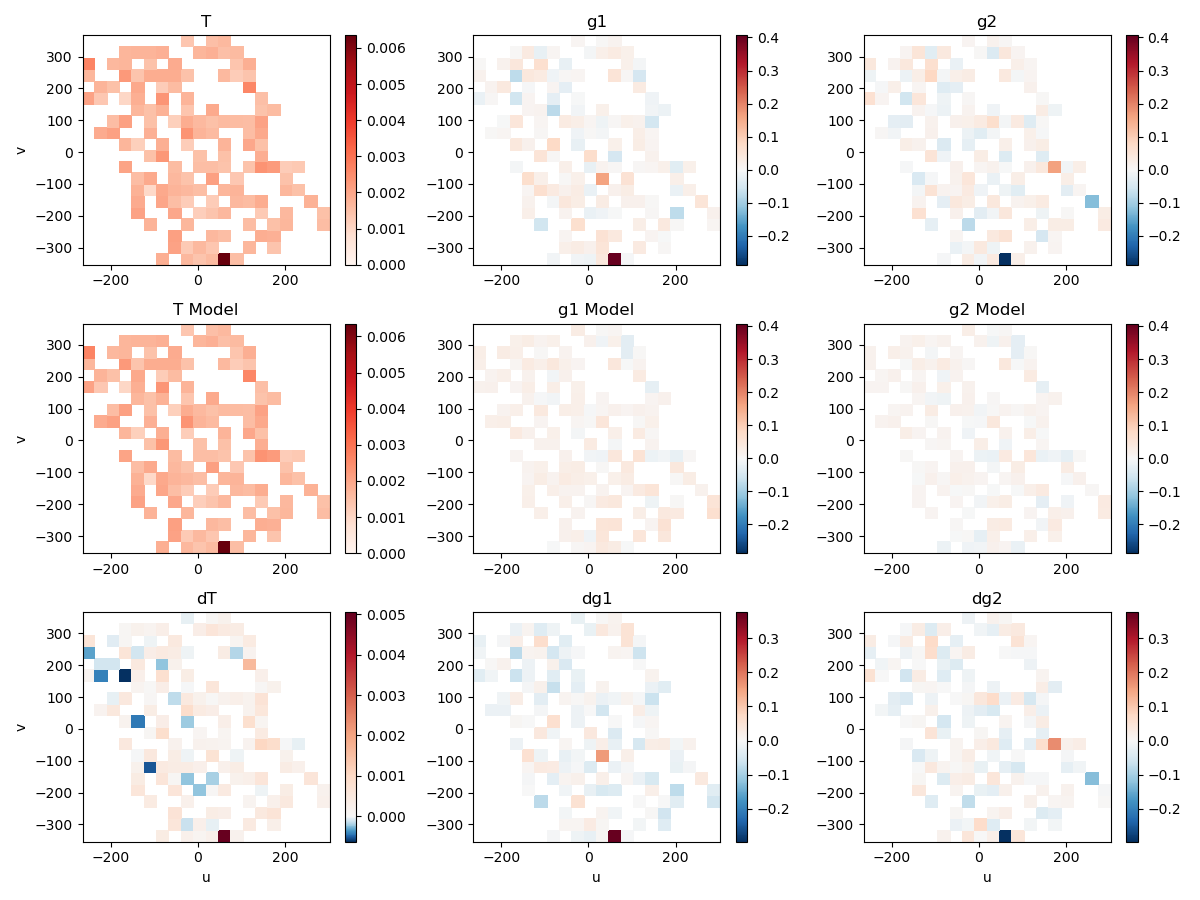
\includegraphics[width=.3\linewidth]{150wControl/piff_twod.png}\hfill
  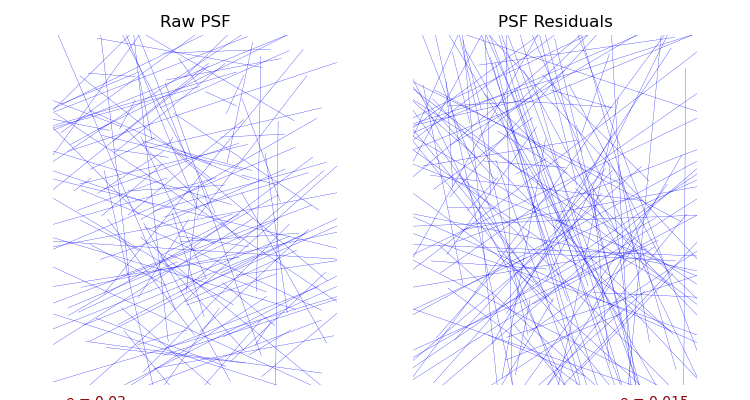
\includegraphics[width=.3\linewidth]{150wControl/piff_whisker.png}\hfill
  \caption{f150w Control}
  \end{subfigure}\par\medskip


\end{figure}\\
\begin{figure}
  \begin{subfigure}{\linewidth}
  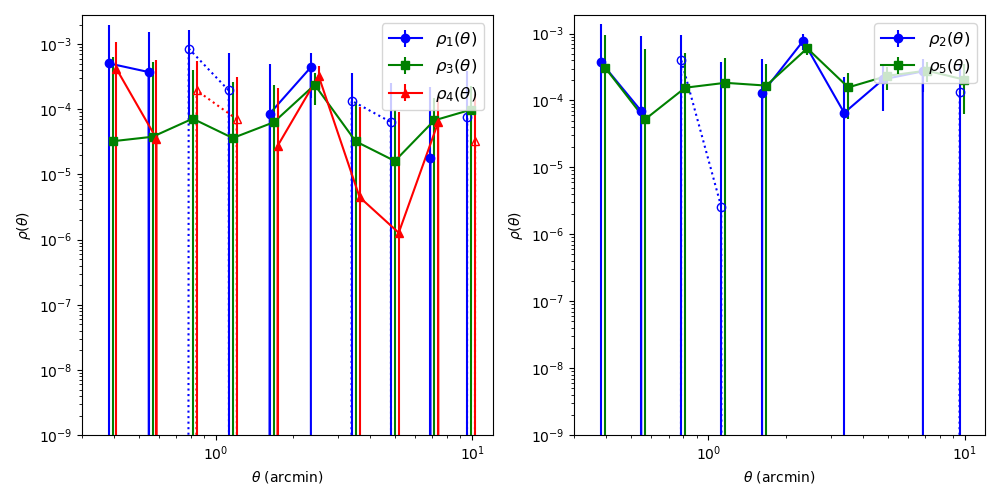
\includegraphics[width=.3\linewidth]{115wControl/piff_rho.png}\hfill
  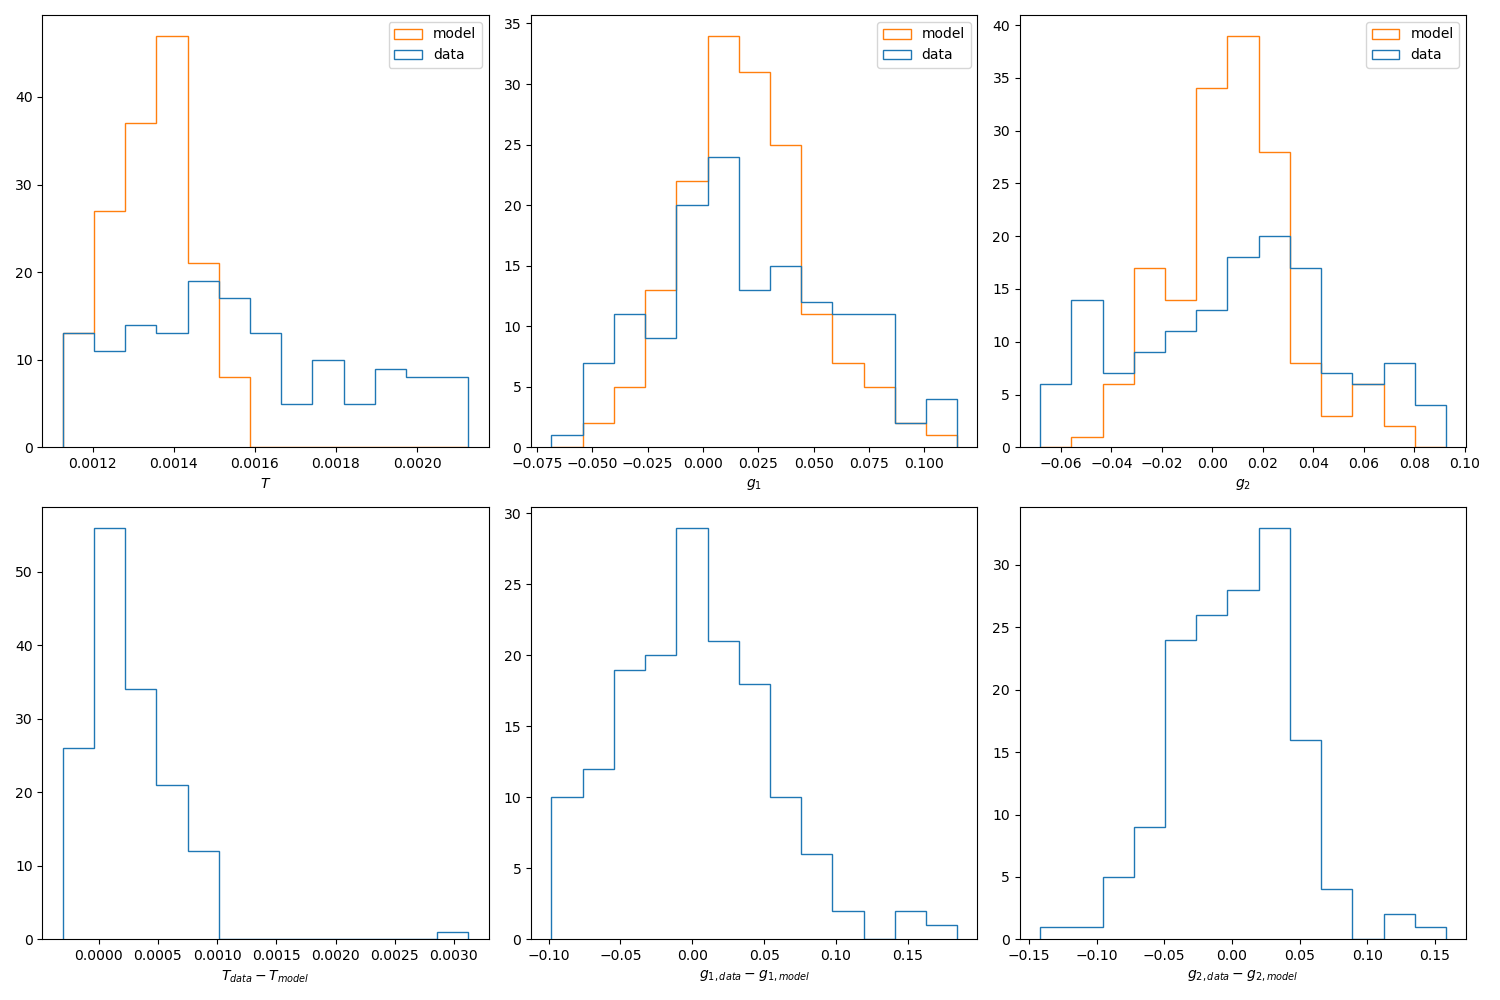
\includegraphics[width=.3\linewidth]{115wControl/piff_shapes.png}\hfill
  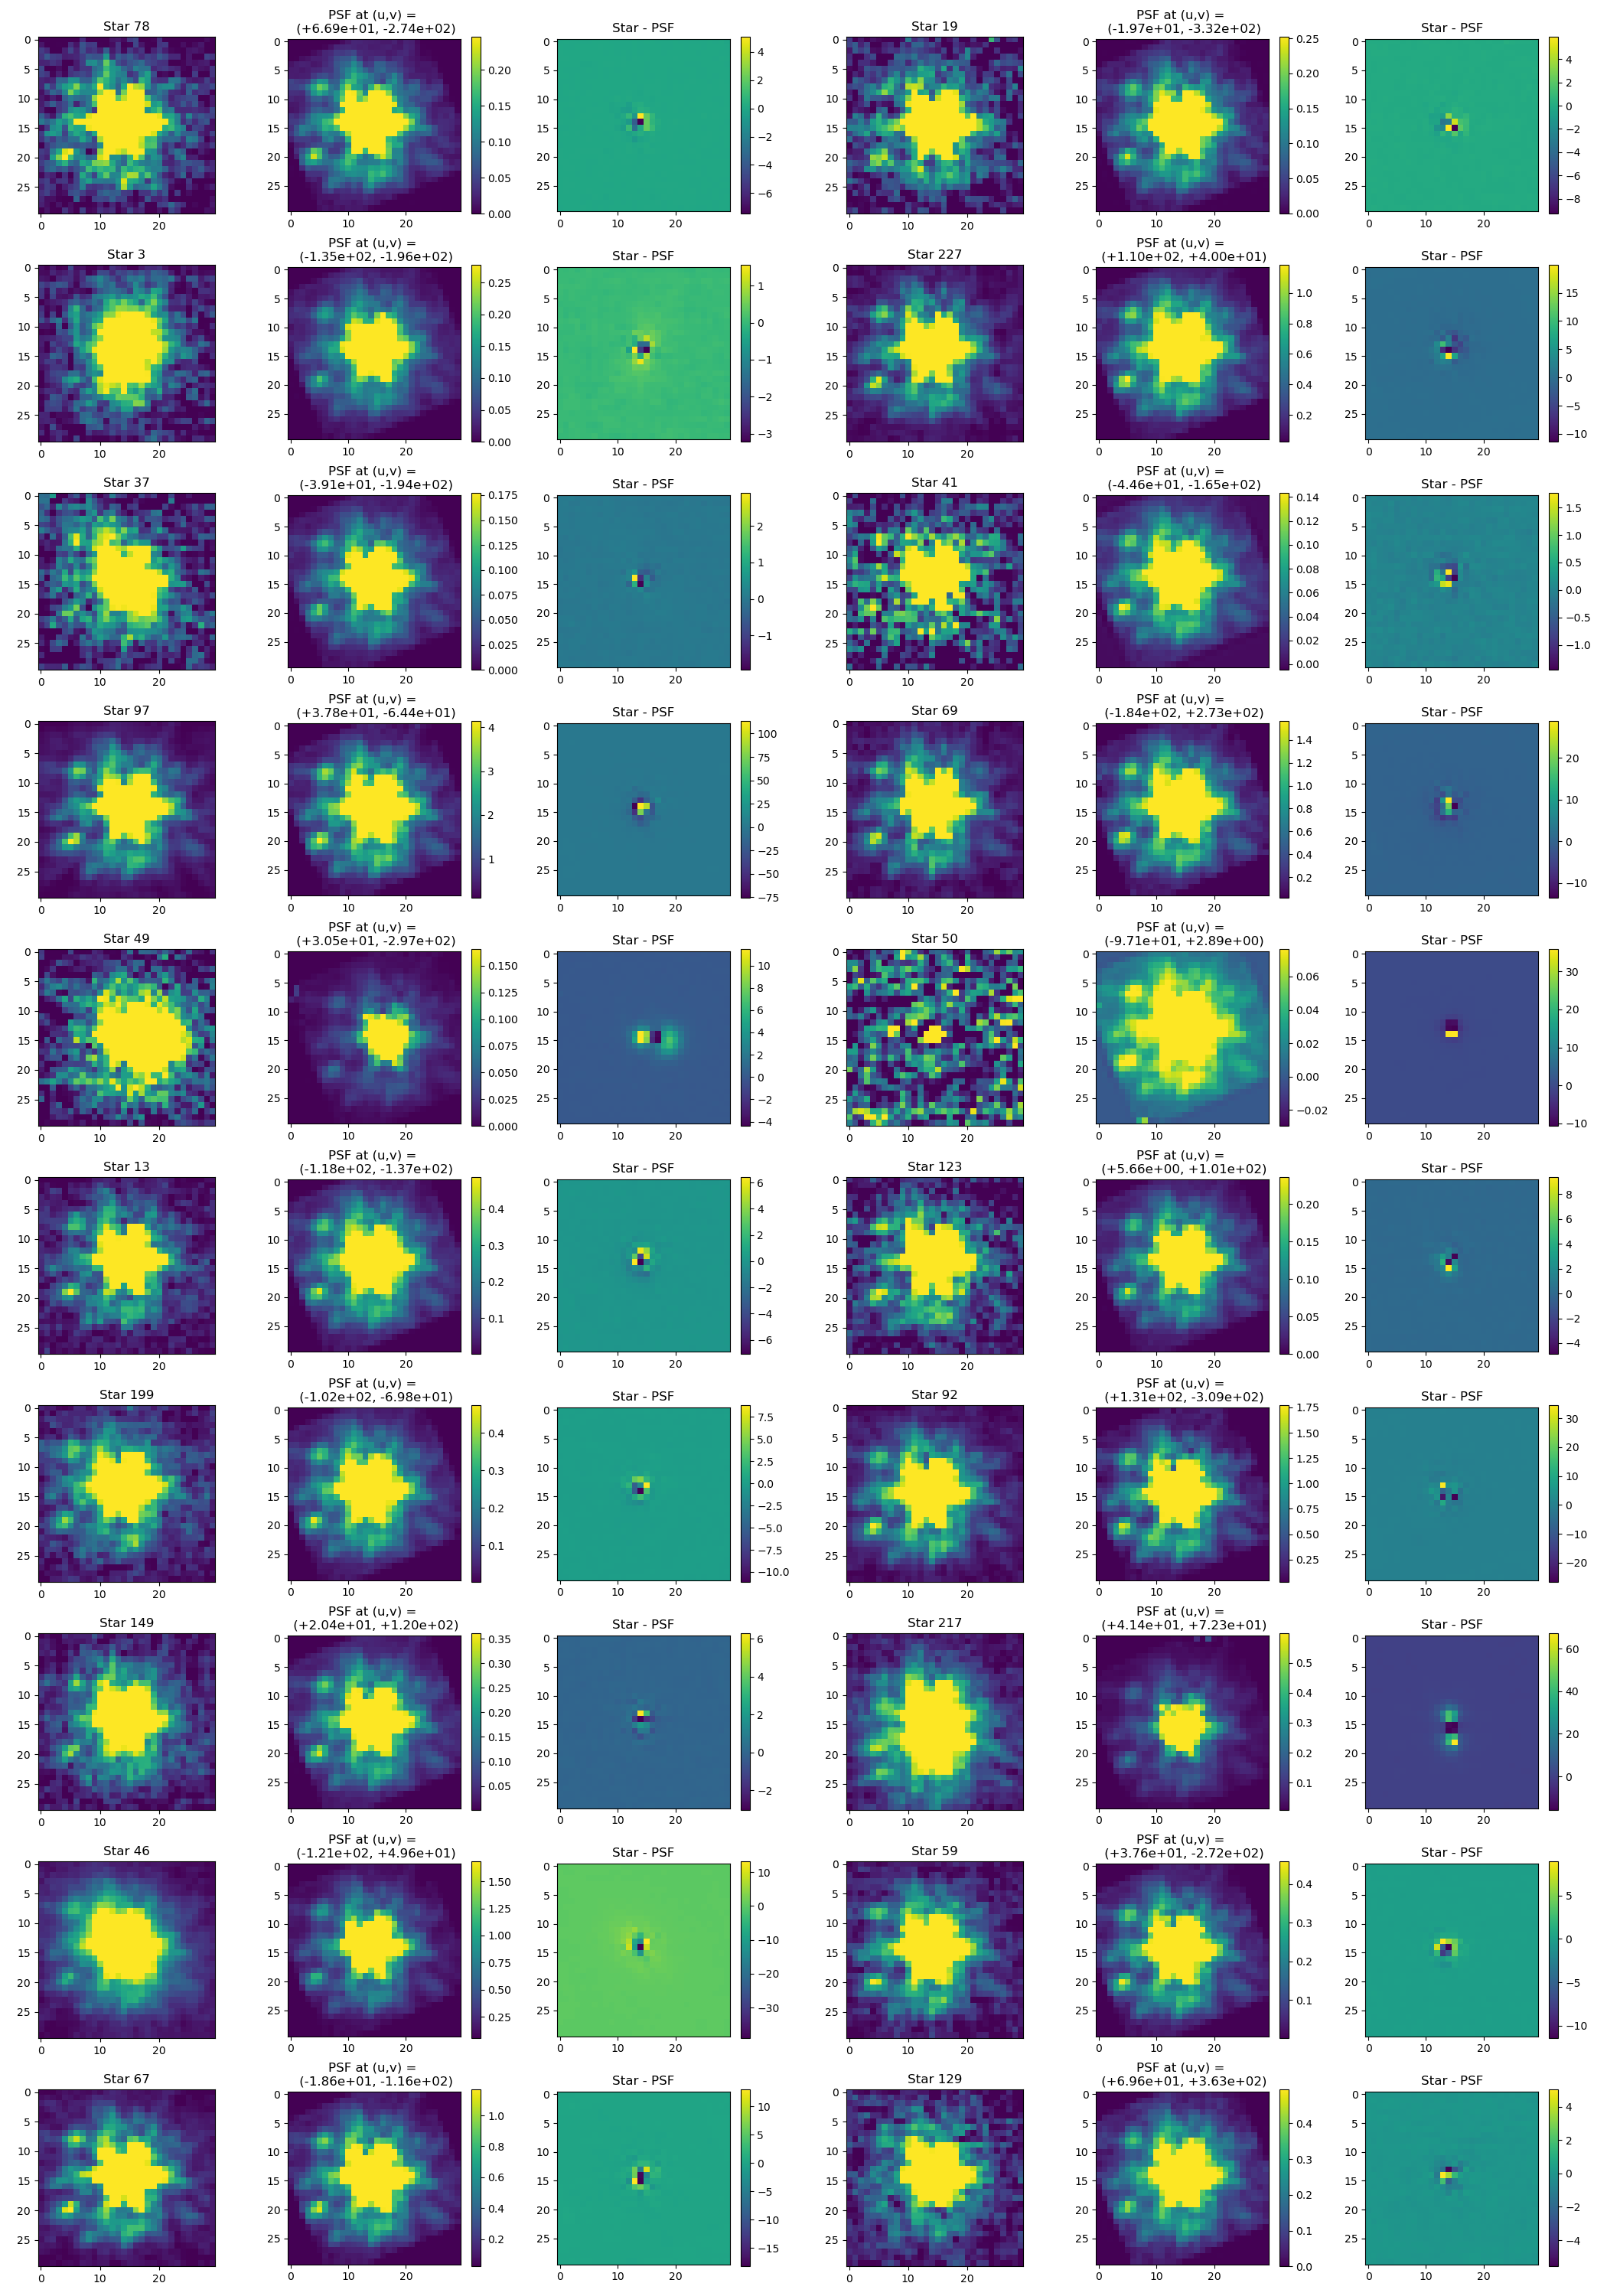
\includegraphics[width=.3\linewidth]{115wControl/piff_stars.png}
  \end{subfigure}\par\medskip
  \begin{subfigure}{\linewidth}
  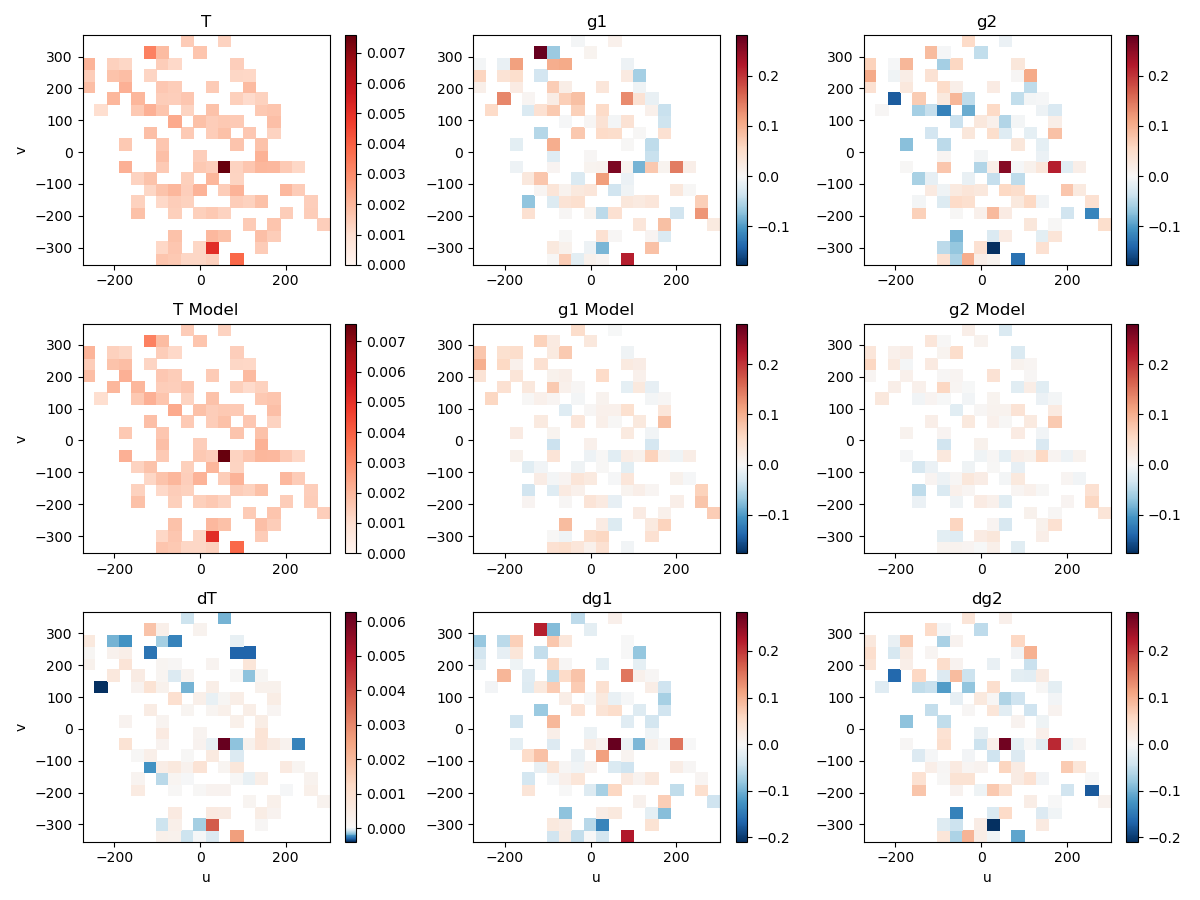
\includegraphics[width=.3\linewidth]{115wControl/piff_twod.png}\hfill
  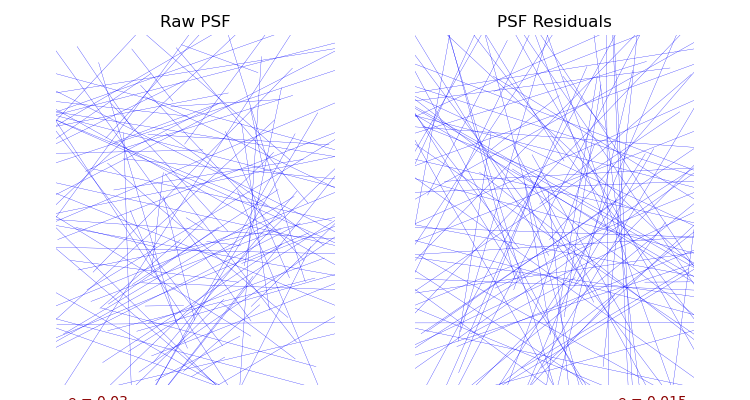
\includegraphics[width=.3\linewidth]{115wControl/piff_whisker.png}\hfill
  \caption{f115w Control}
  \end{subfigure}\par\medskip


\end{figure}
\begin{figure}
  \begin{subfigure}{\linewidth}
  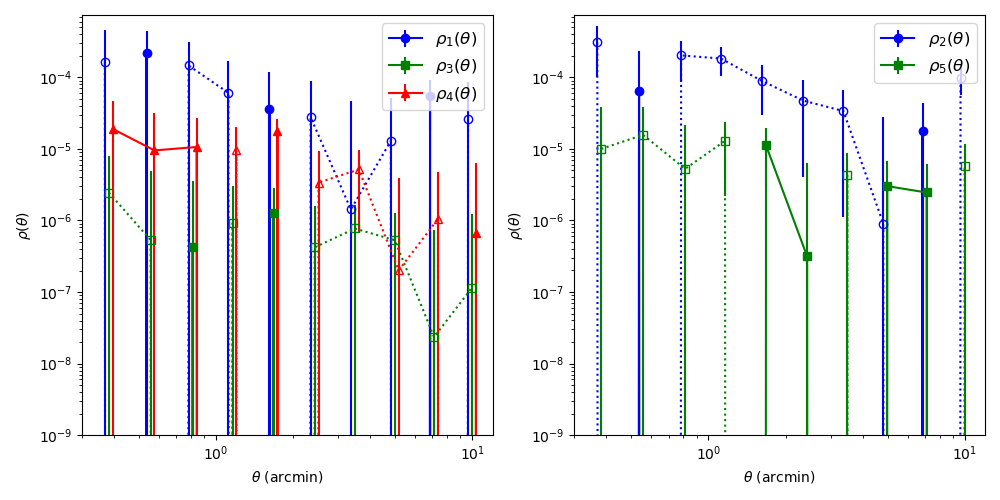
\includegraphics[width=.3\linewidth]{227wControl/piff_rho.png}\hfill
  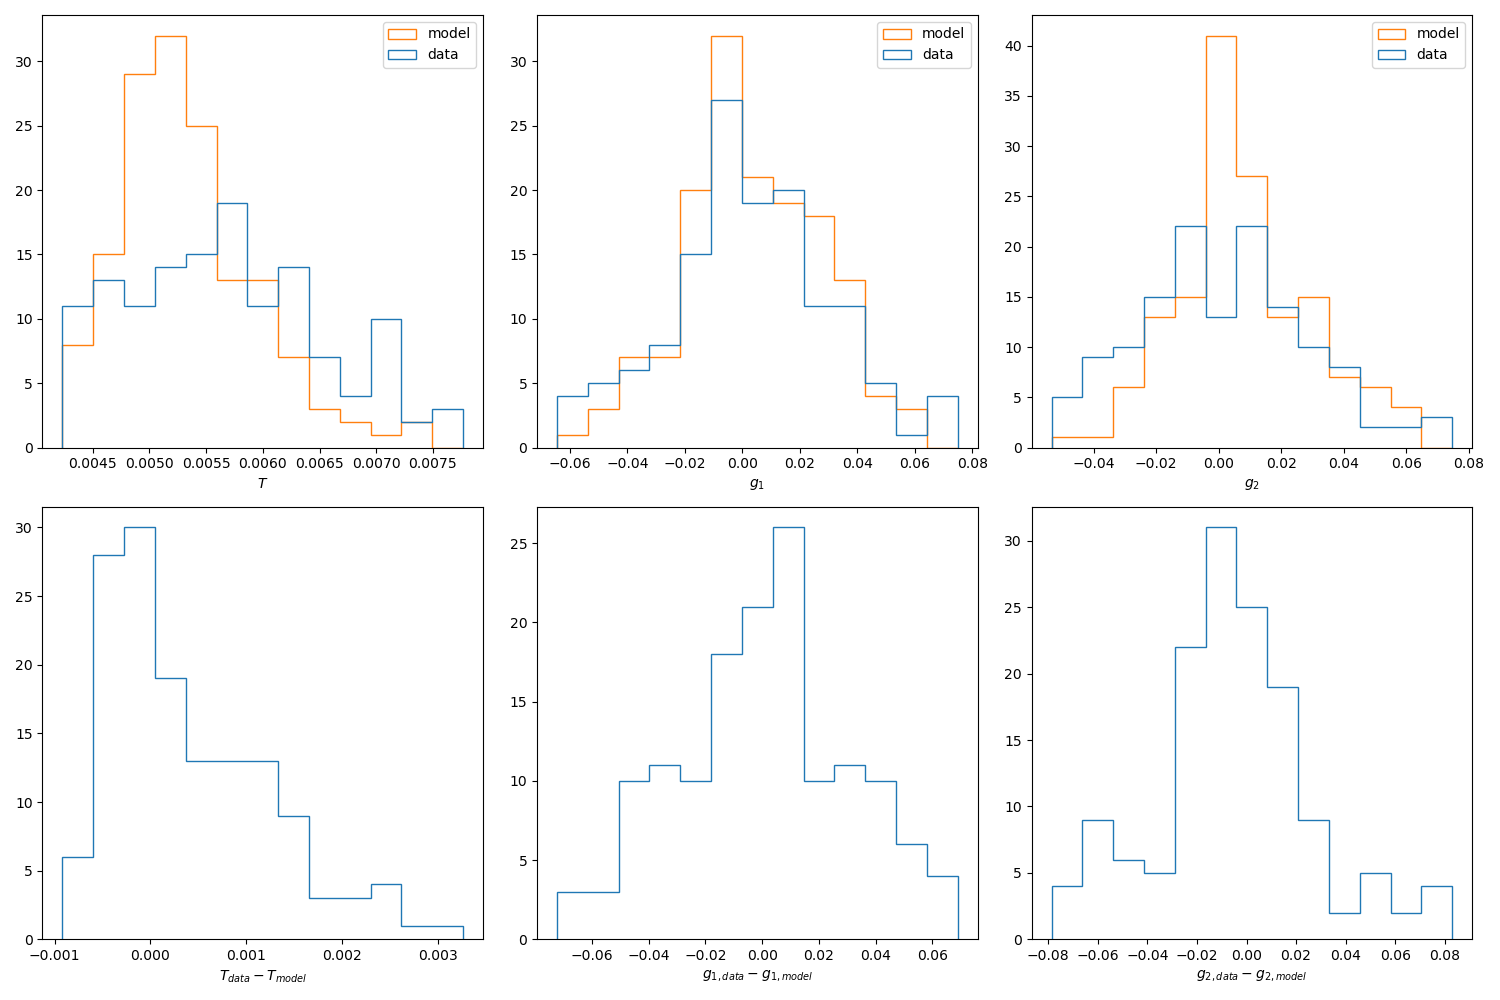
\includegraphics[width=.3\linewidth]{227wControl/piff_shapes.png}\hfill
  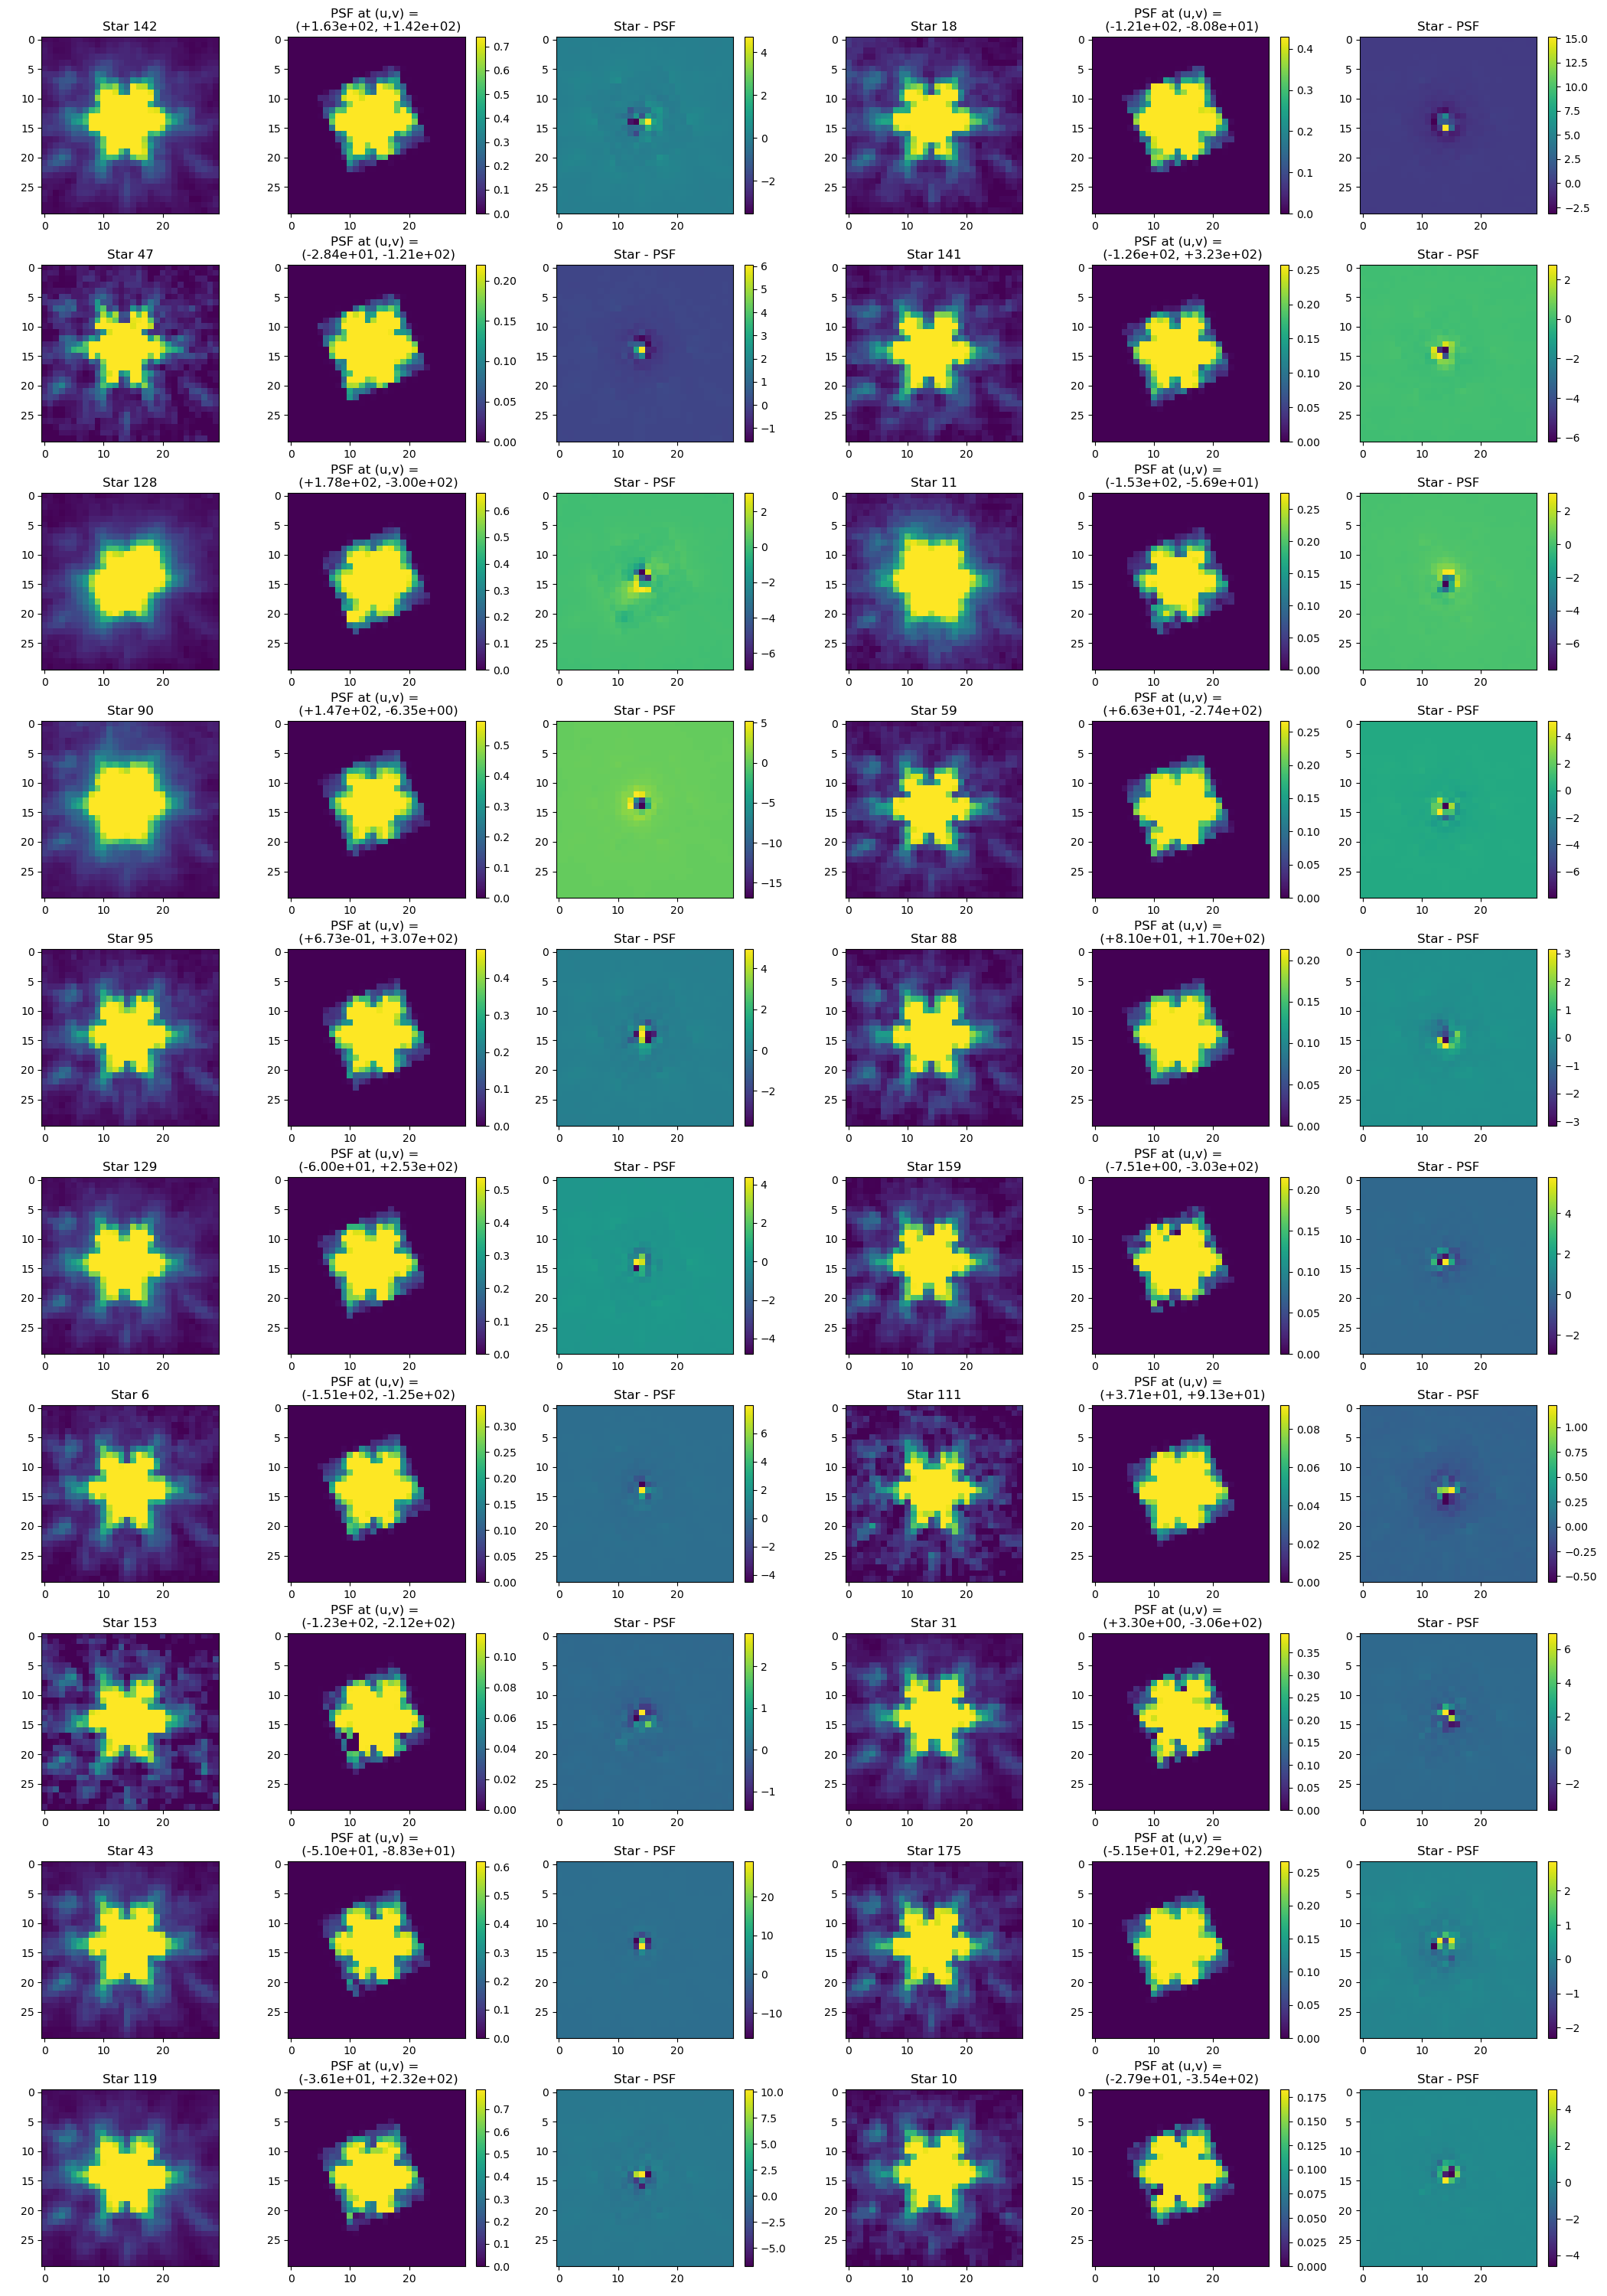
\includegraphics[width=.3\linewidth]{227wControl/piff_stars.png}
  \end{subfigure}\par\medskip
  \begin{subfigure}{\linewidth}
  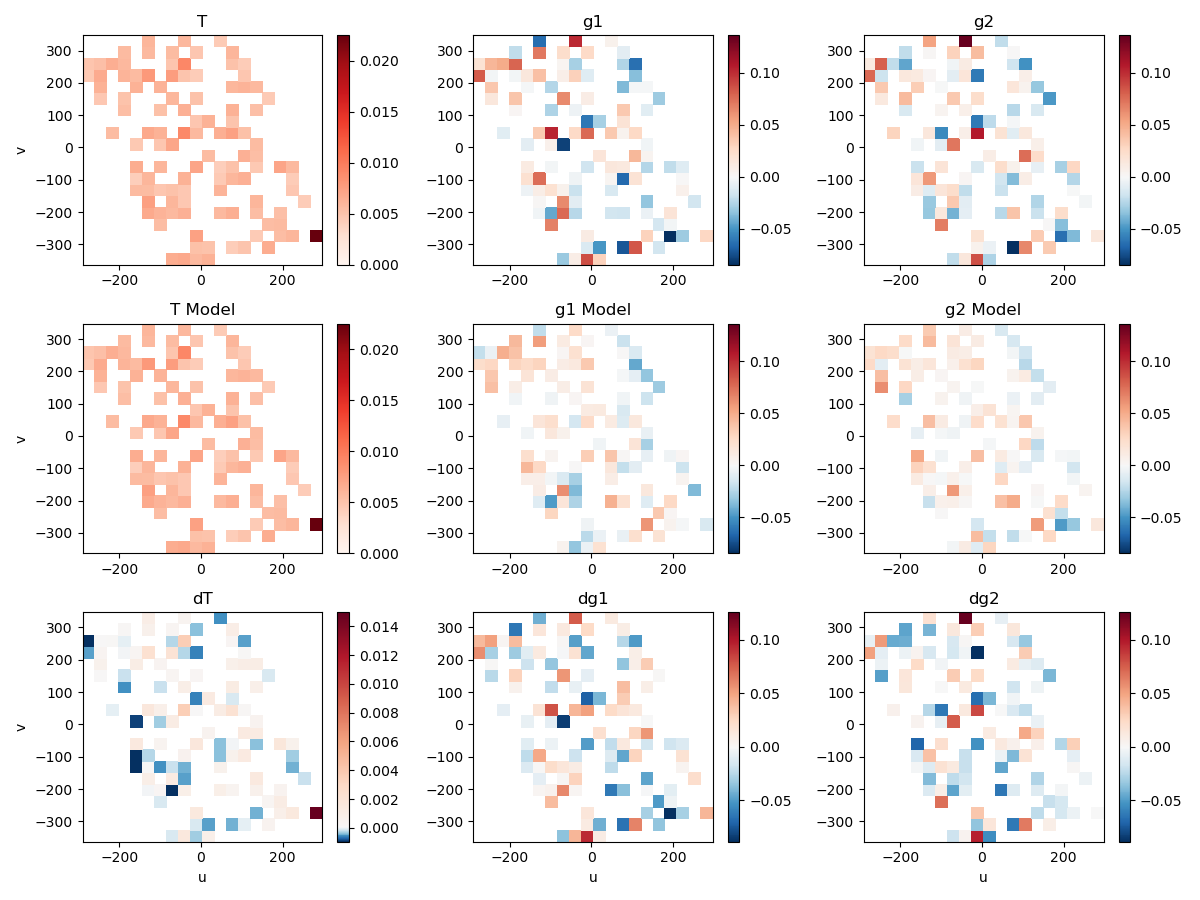
\includegraphics[width=.3\linewidth]{227wControl/piff_twod.png}\hfill
  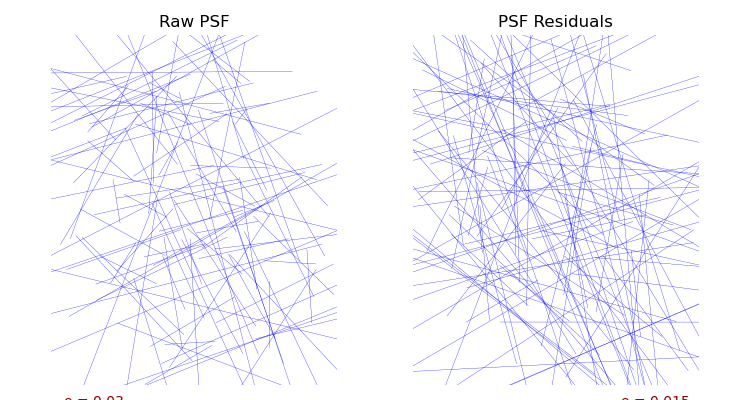
\includegraphics[width=.3\linewidth]{227wControl/piff_whisker.png}\hfill
  \caption{f227w Control}
  \end{subfigure}\par\medskip


\end{figure}

\begin{figure}
  \begin{subfigure}{\linewidth}
  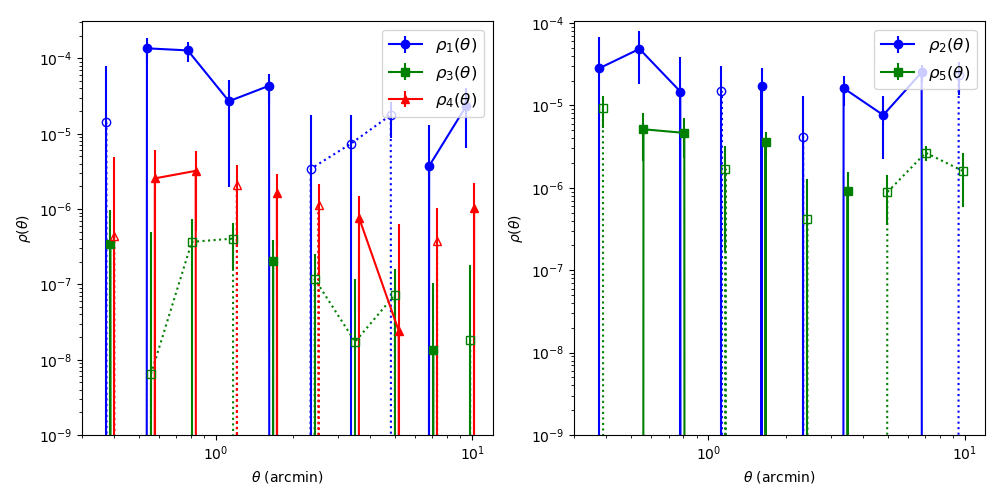
\includegraphics[width=.3\linewidth]{444wControl/piff_rho.png}\hfill
  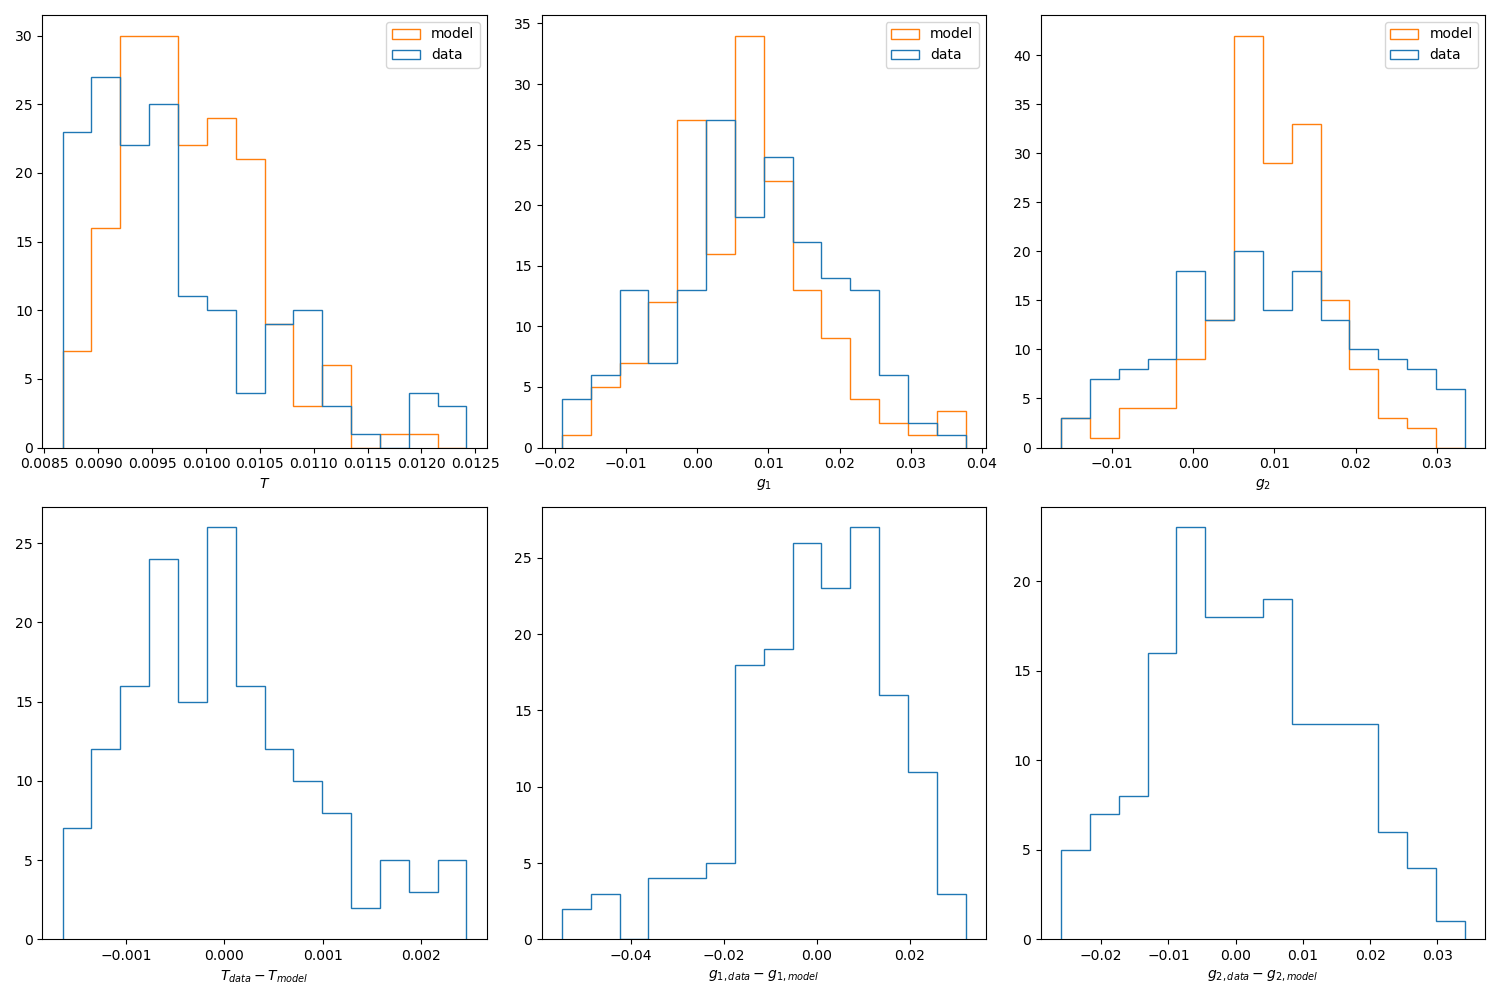
\includegraphics[width=.3\linewidth]{444wControl/piff_shapes.png}\hfill
  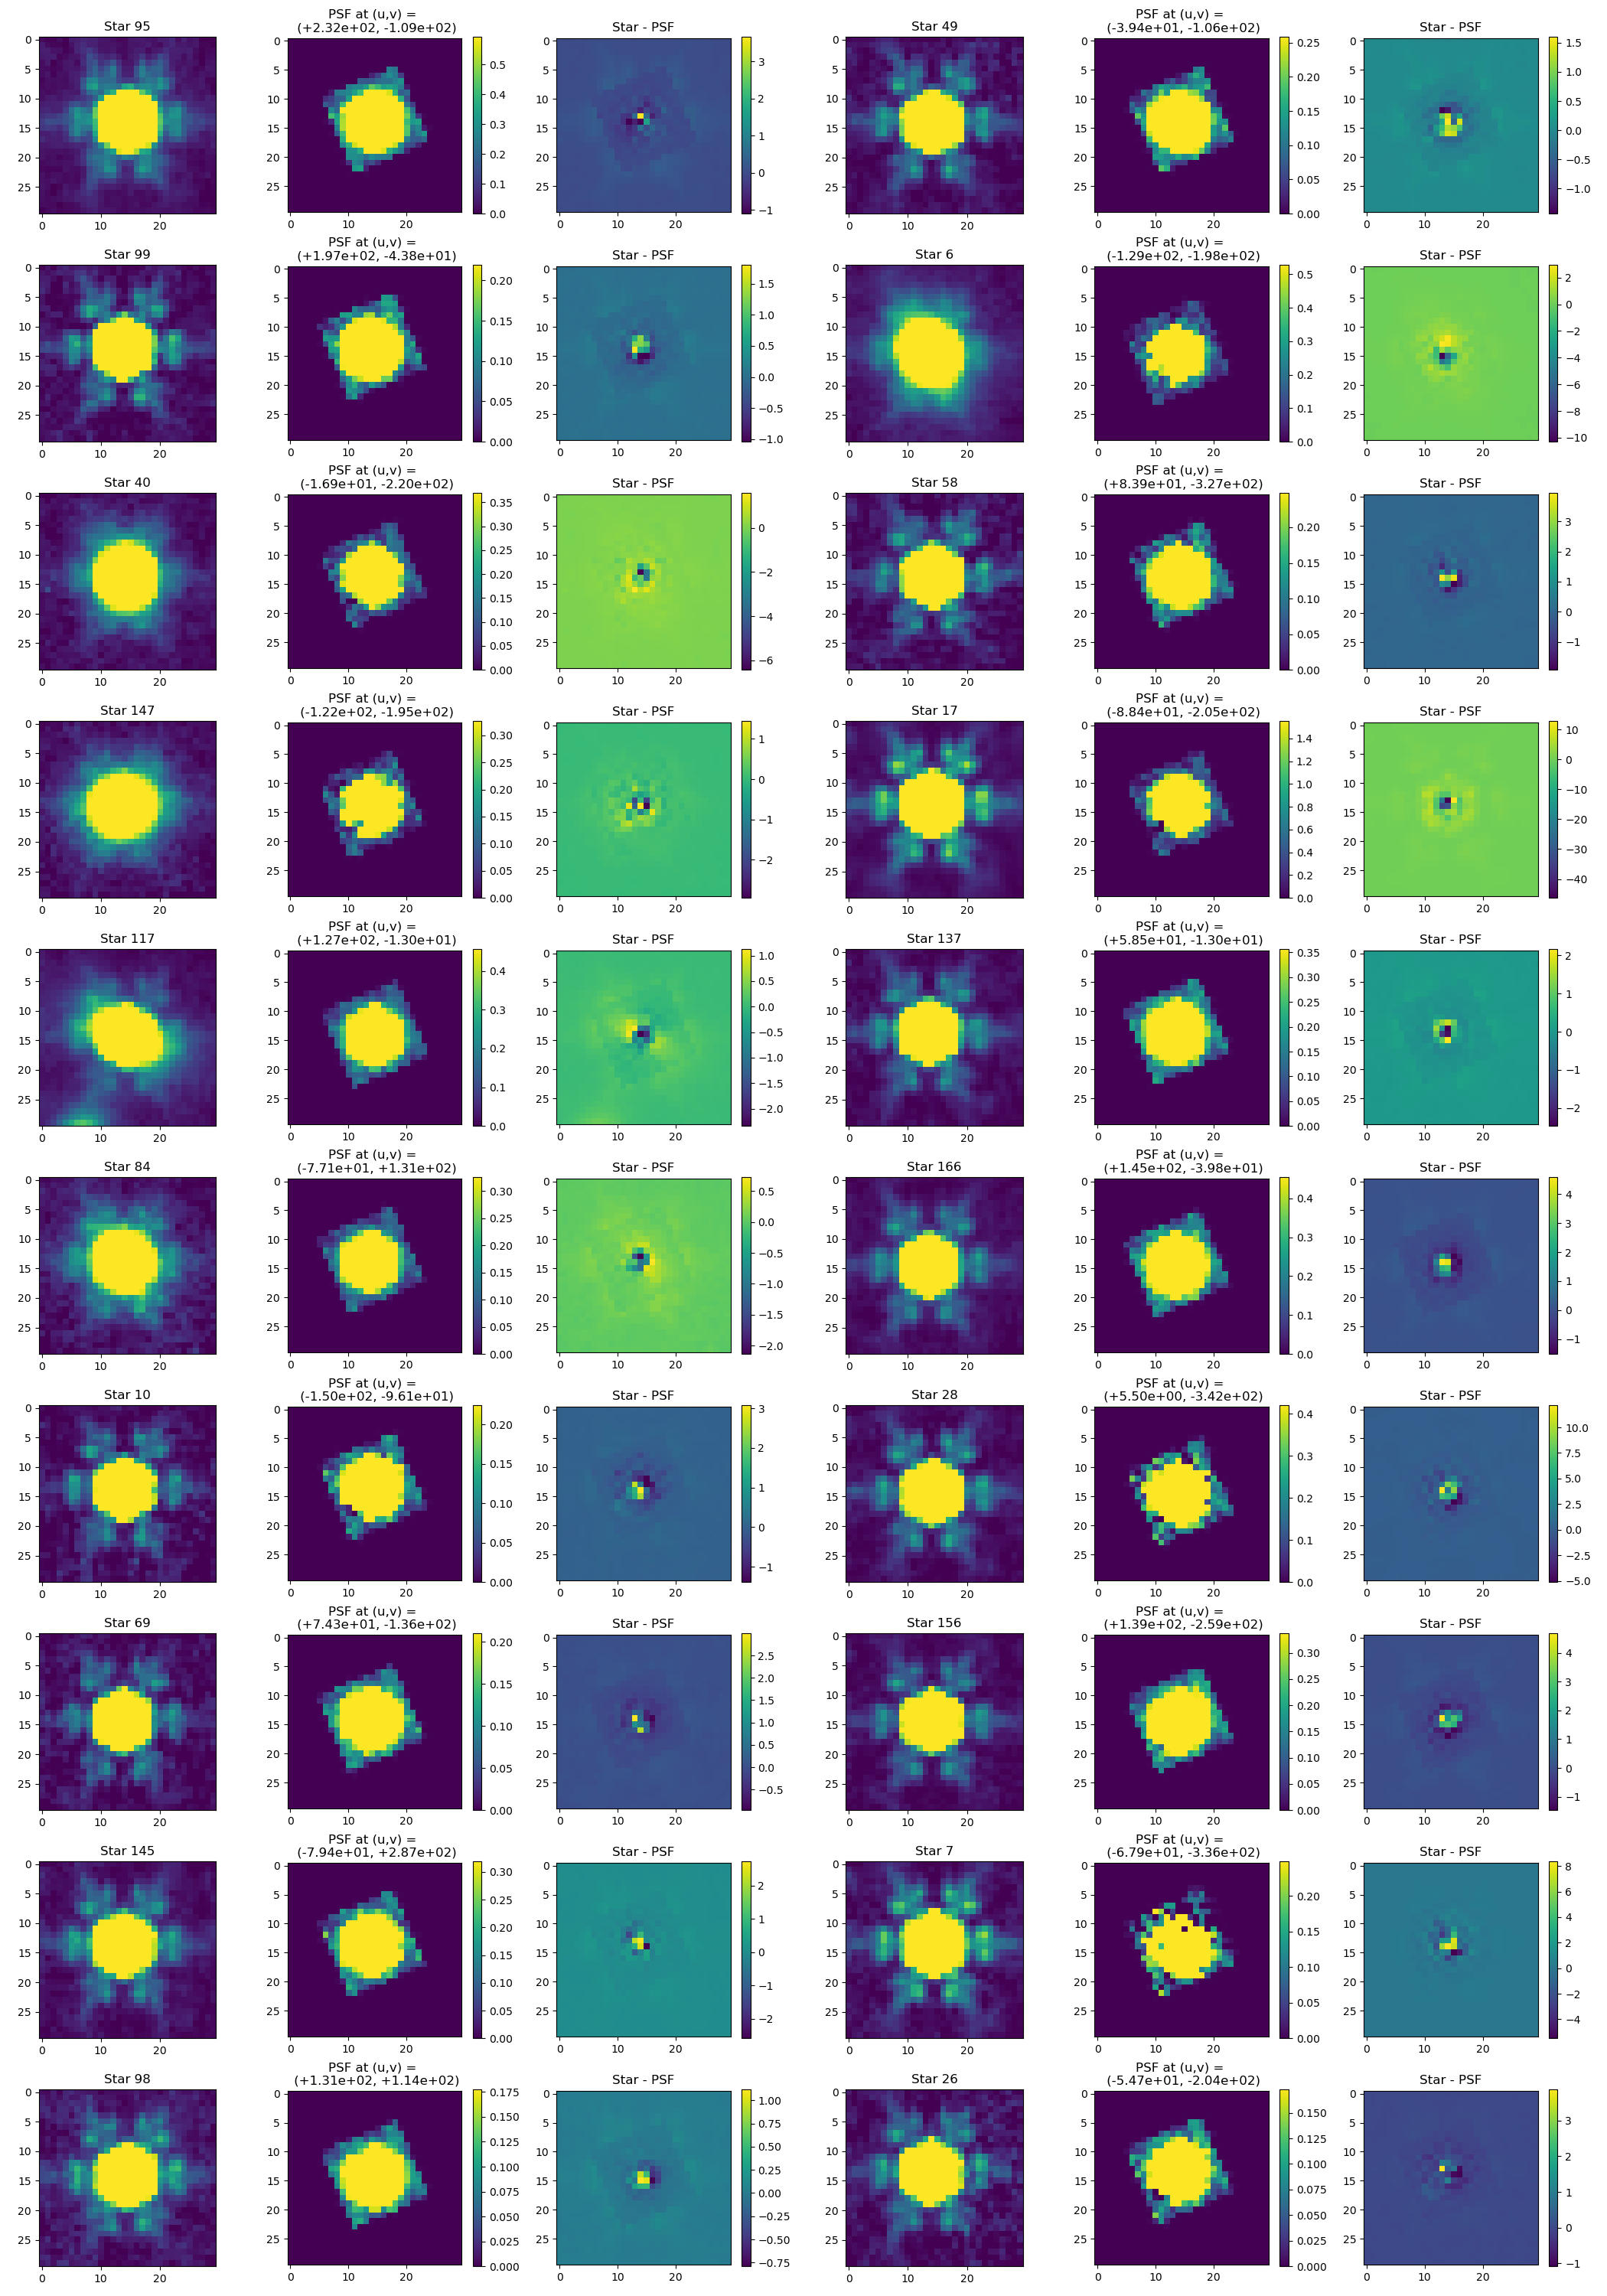
\includegraphics[width=.3\linewidth]{444wControl/piff_stars.png}
  \end{subfigure}\par\medskip
  \begin{subfigure}{\linewidth}
  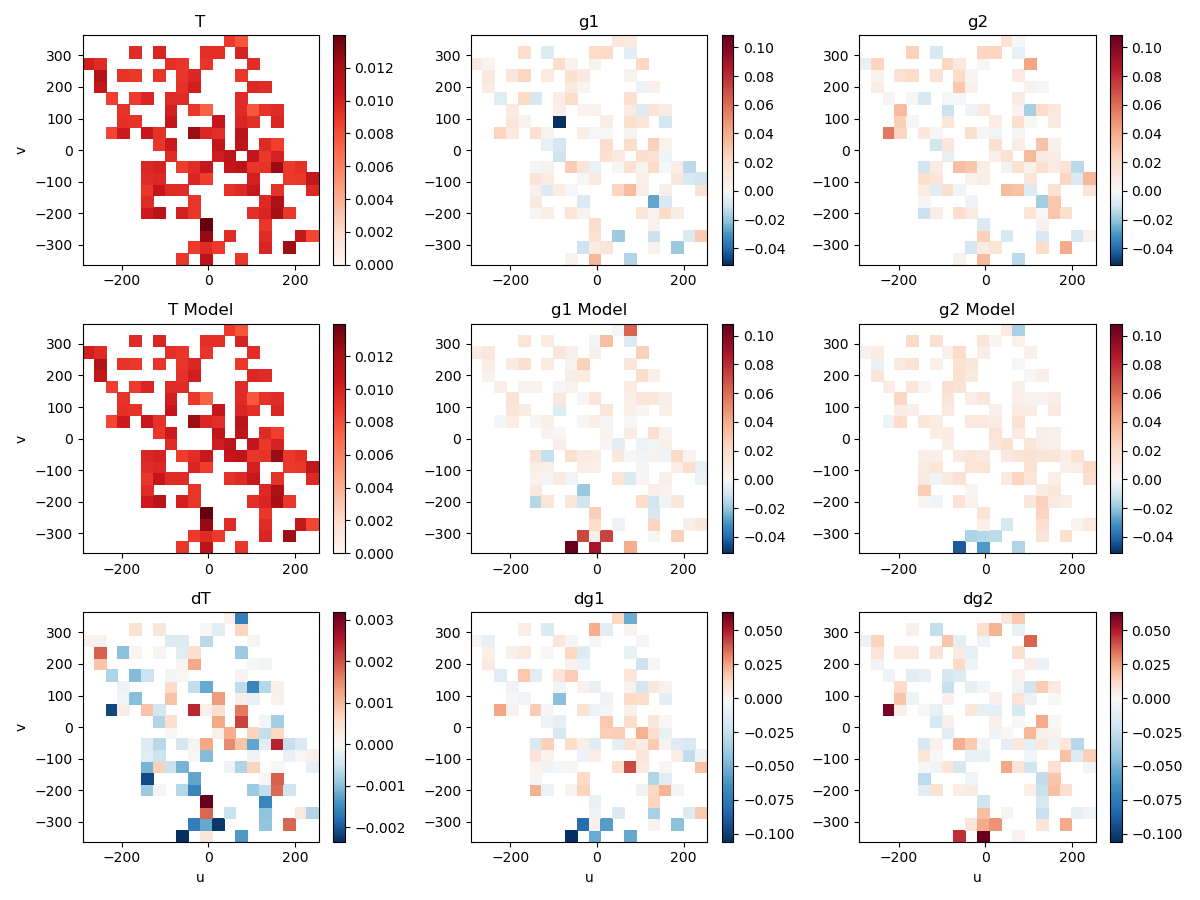
\includegraphics[width=.3\linewidth]{444wControl/piff_twod.png}\hfill
  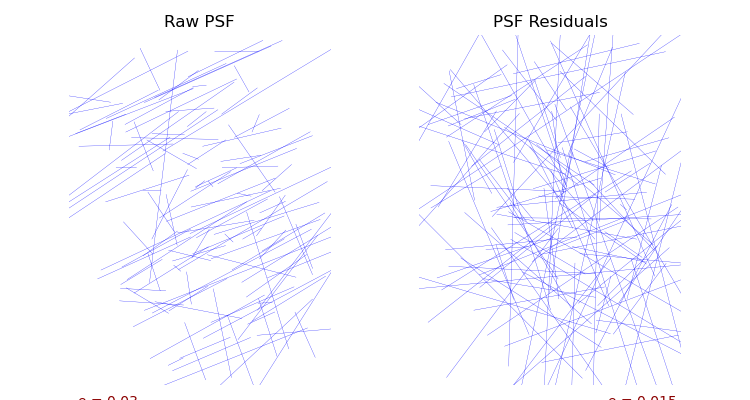
\includegraphics[width=.3\linewidth]{444wControl/piff_whisker.png}\hfill
  \caption{f444w Control}
  \end{subfigure}\par\medskip


\end{figure}\\ \newpage

\begin{python}
# How large should the postage stamp cutouts of the stars be?
    stamp_size: 30

model:
    # This model uses a grid of pixels to model the surface brightness distribution.
    type: PixelGrid
    scale: 0.025      # NIRCam ative pixel scale
    size: 19          # Model is 24 x 24 in these
\end{python}\\
\begin{figure}[!h]
  \begin{subfigure}{\linewidth}
  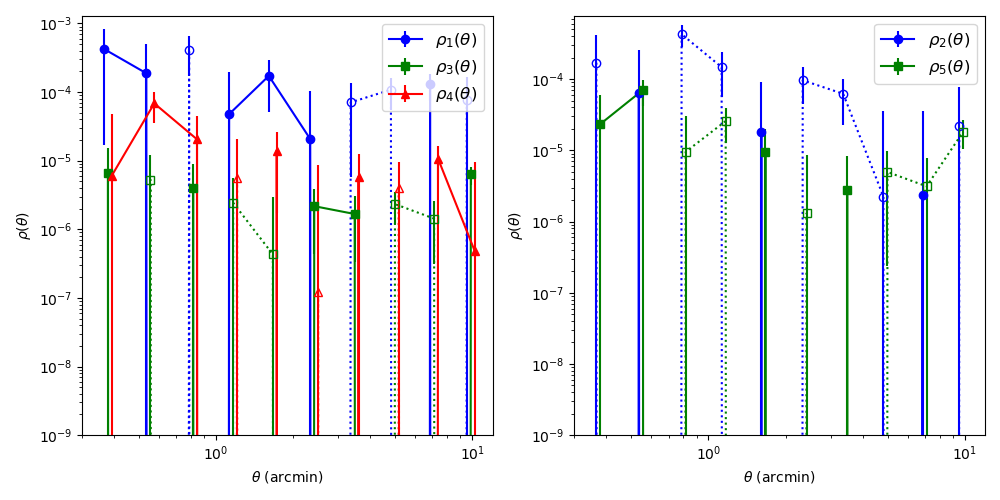
\includegraphics[width=.3\linewidth]{227wFiner/piff_rho.png}\hfill
  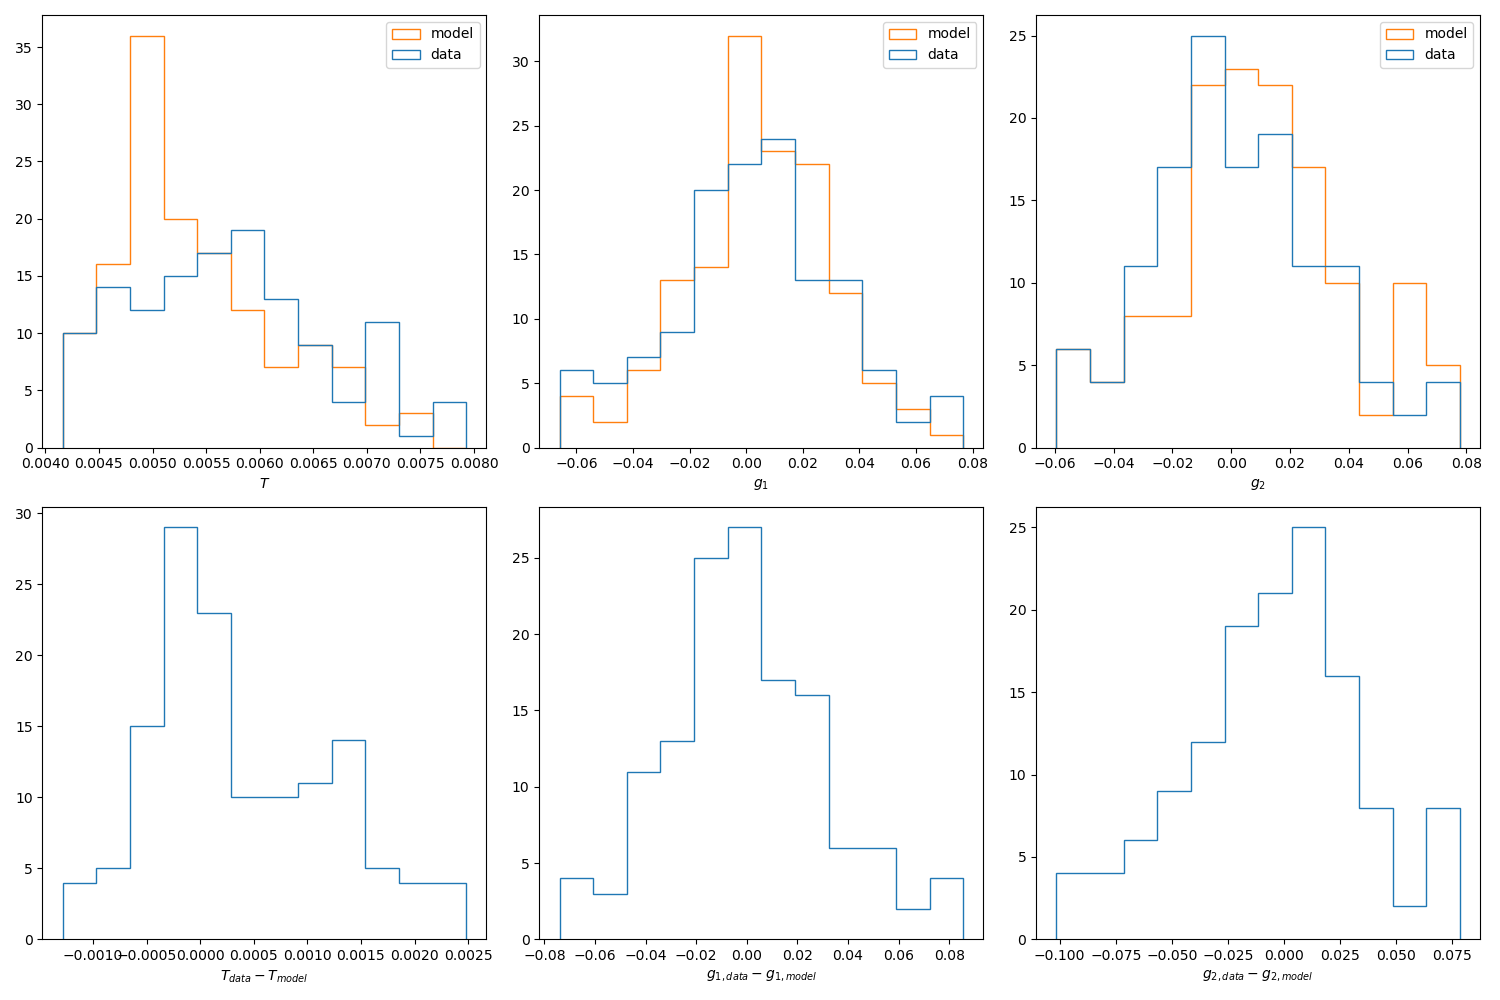
\includegraphics[width=.3\linewidth]{227wFiner/piff_shapes.png}\hfill
  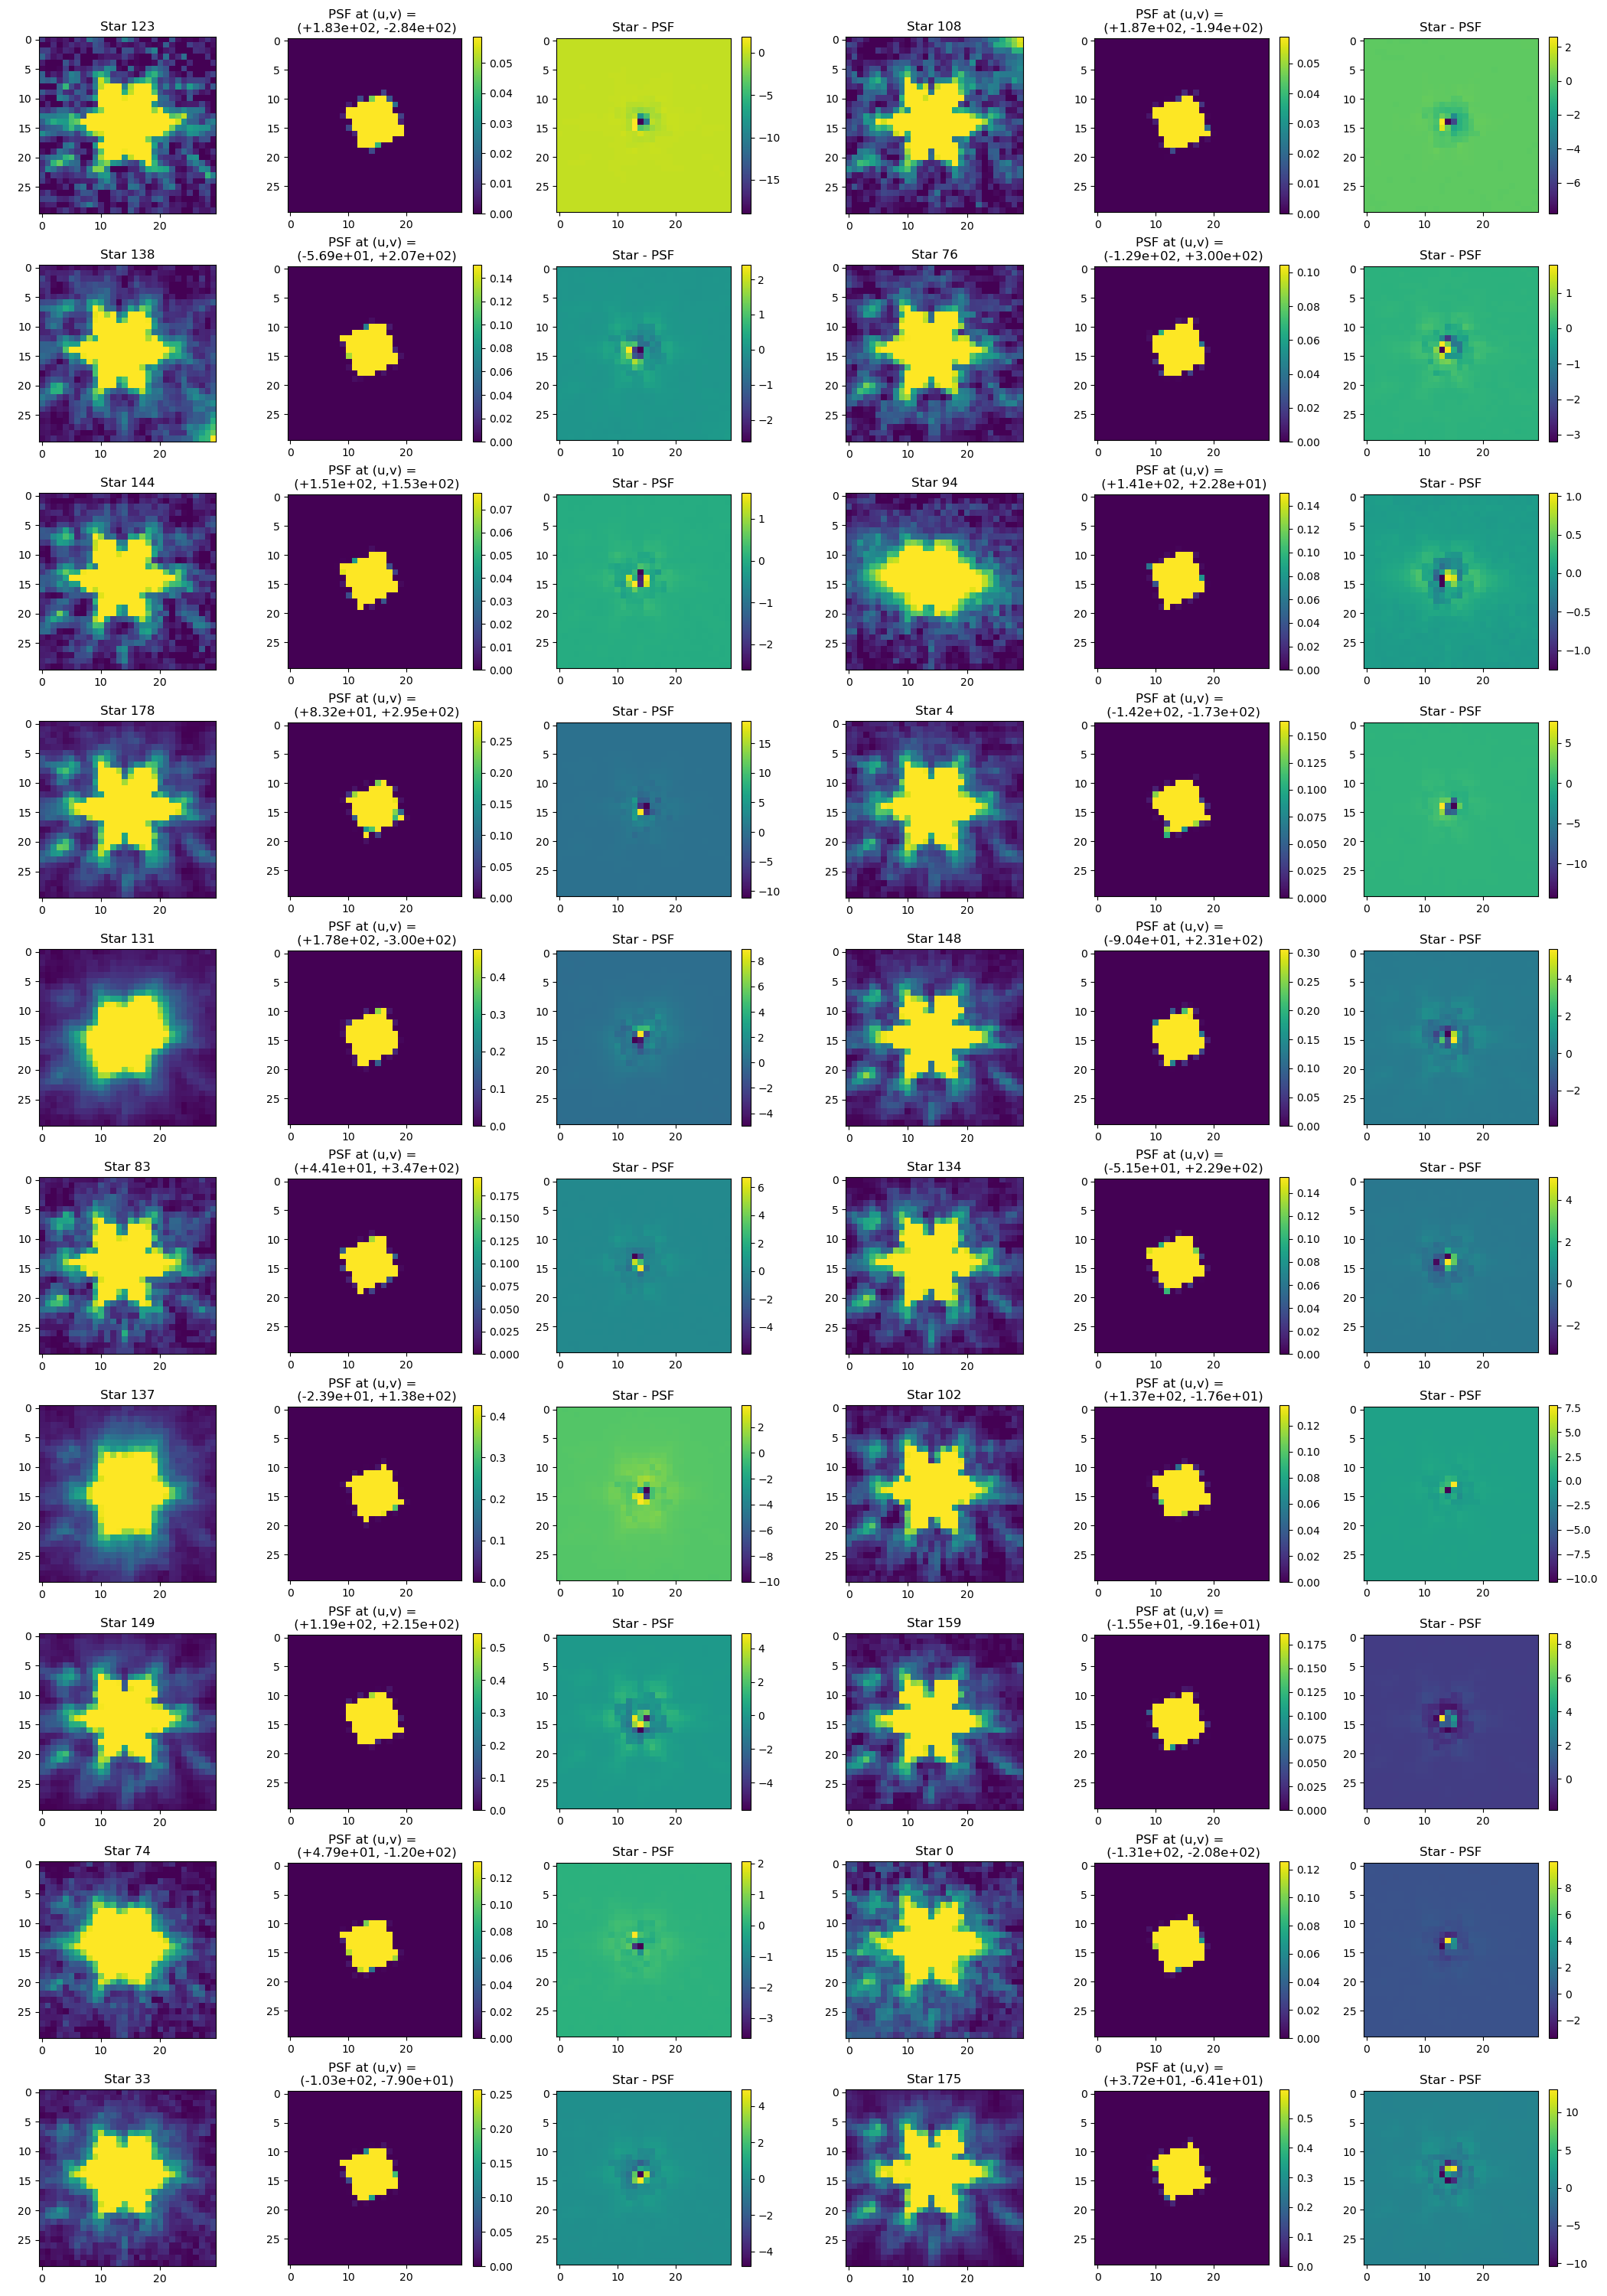
\includegraphics[width=.3\linewidth]{227wFiner/piff_stars.png}
  \end{subfigure}\par\medskip
  \begin{subfigure}{\linewidth}
  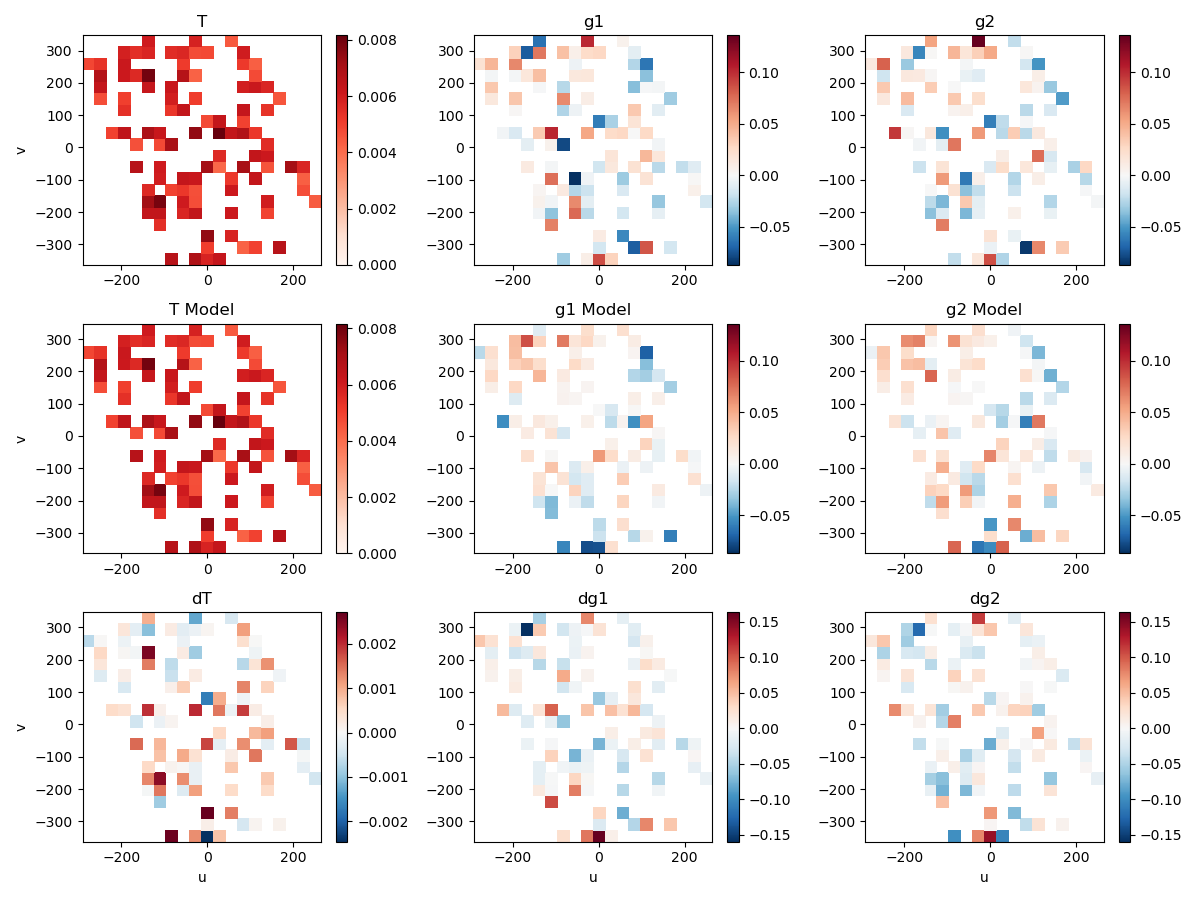
\includegraphics[width=.3\linewidth]{227wFiner/piff_twod.png}\hfill
  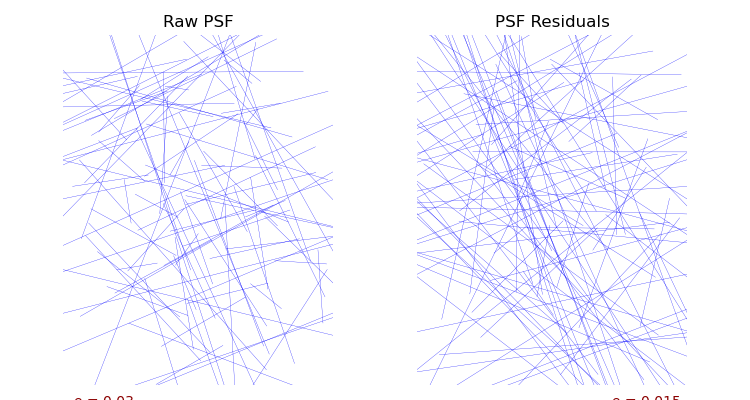
\includegraphics[width=.3\linewidth]{227wFiner/piff_whisker.png}\hfill
  \caption{f227w Finer}
  \end{subfigure}\par\medskip


\end{figure} \newpage

\begin{python}
# How large should the postage stamp cutouts of the stars be?
    stamp_size: 30

model:
    # This model uses a grid of pixels to model the surface brightness distribution.
    type: PixelGrid
    scale: 0.030      # NIRCam ative pixel scale
    size: 22          # Model is 24 x 24 in these
\end{python}\\
\begin{figure}[!h]
  \begin{subfigure}{\linewidth}
  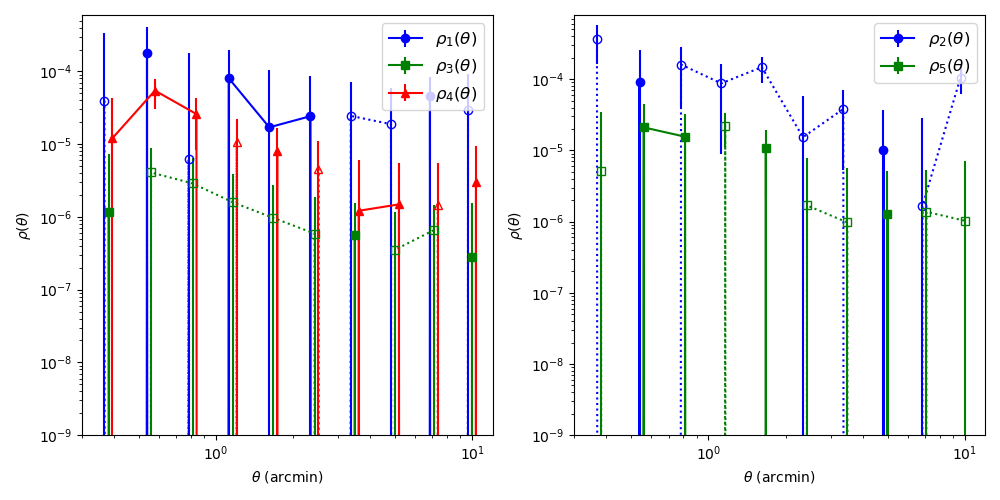
\includegraphics[width=.3\linewidth]{227wMedium/piff_rho.png}\hfill
  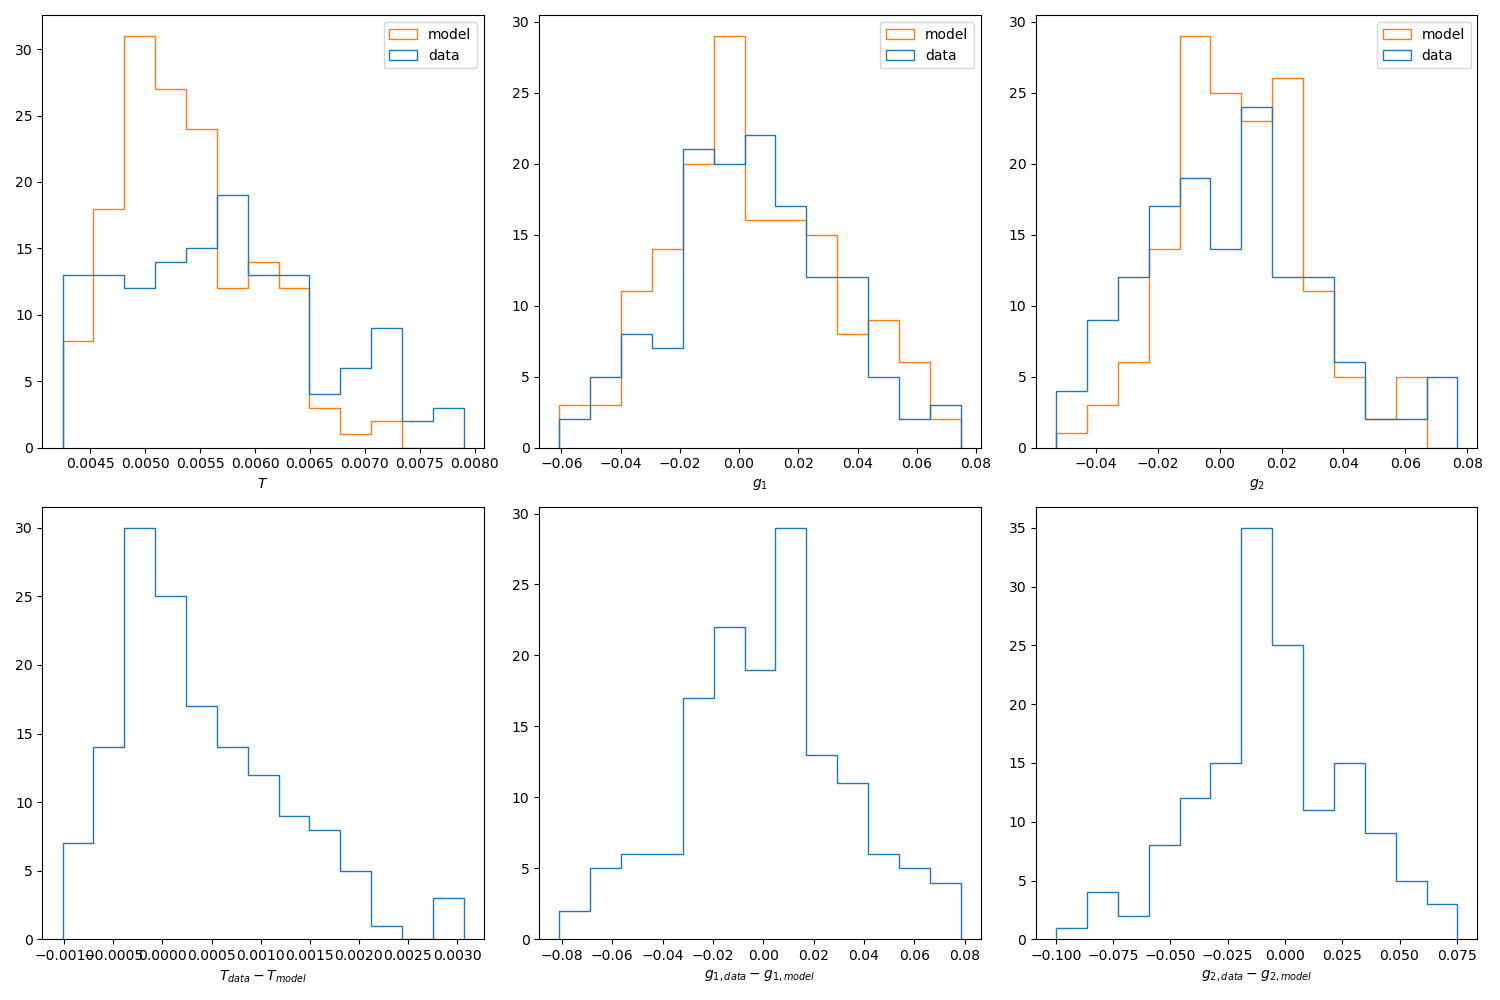
\includegraphics[width=.3\linewidth]{227wMedium/piff_shapes.png}\hfill
  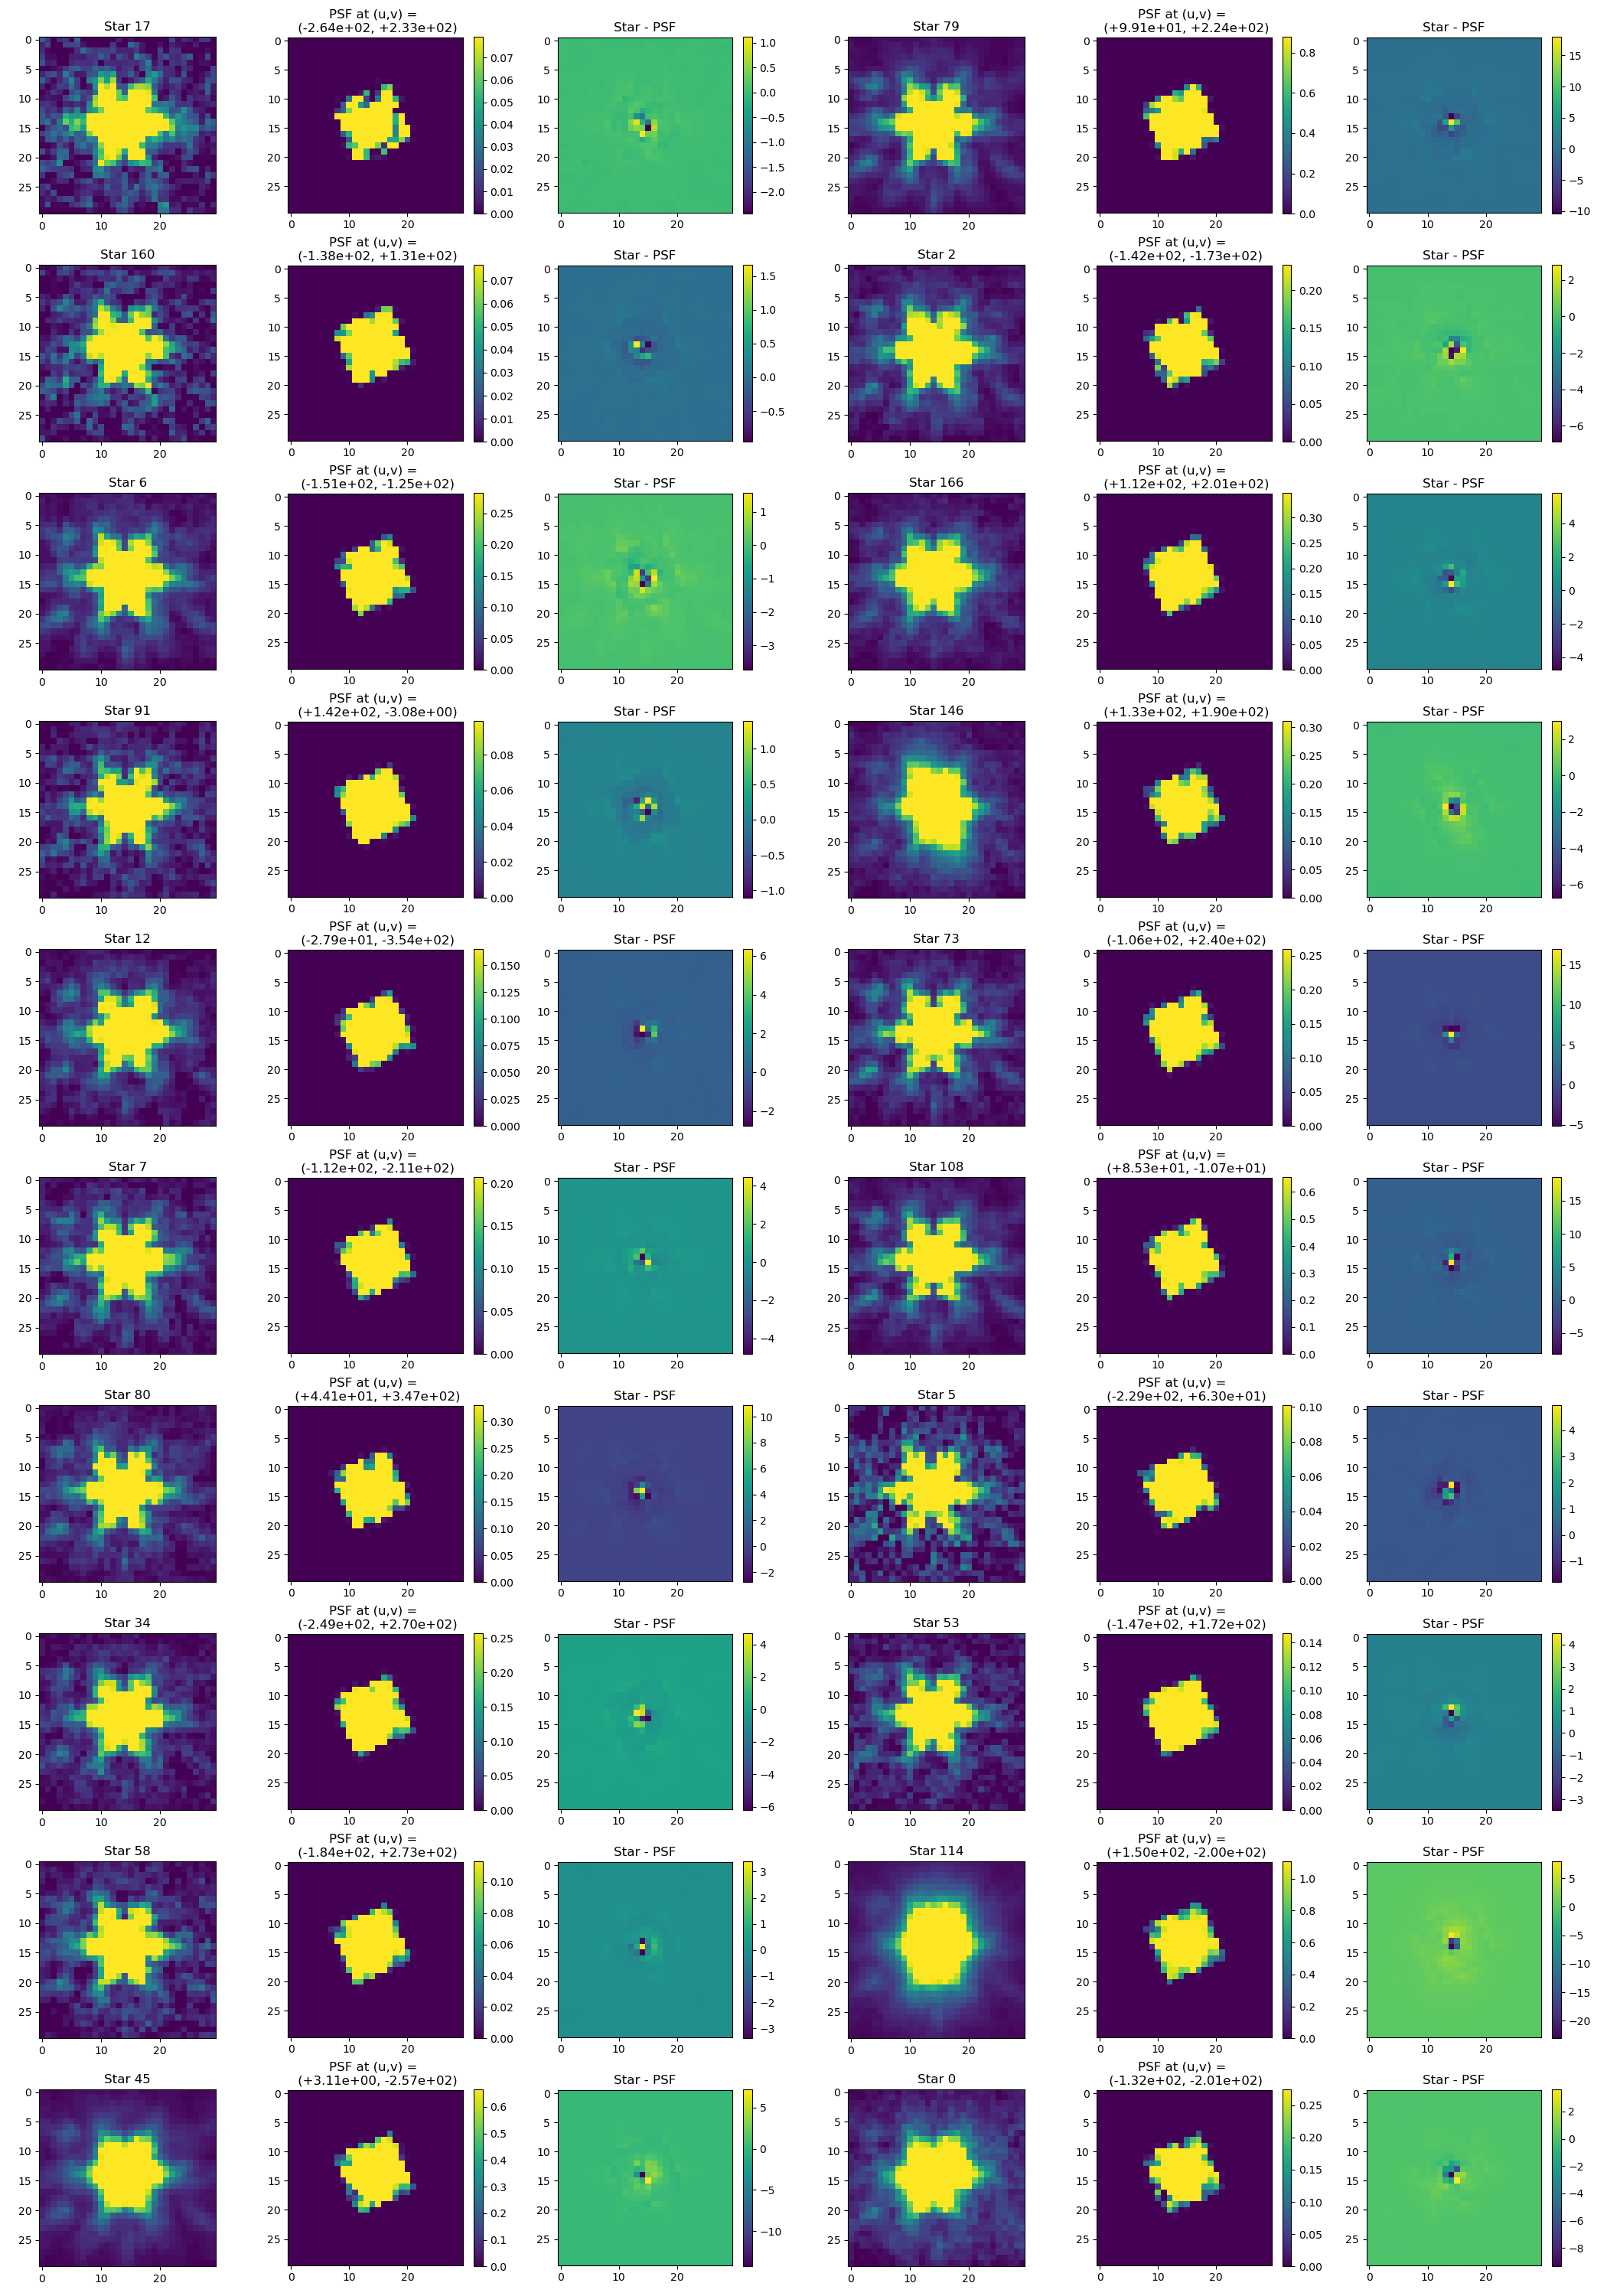
\includegraphics[width=.3\linewidth]{227wMedium/piff_stars.png}
  \end{subfigure}\par\medskip
  \begin{subfigure}{\linewidth}
  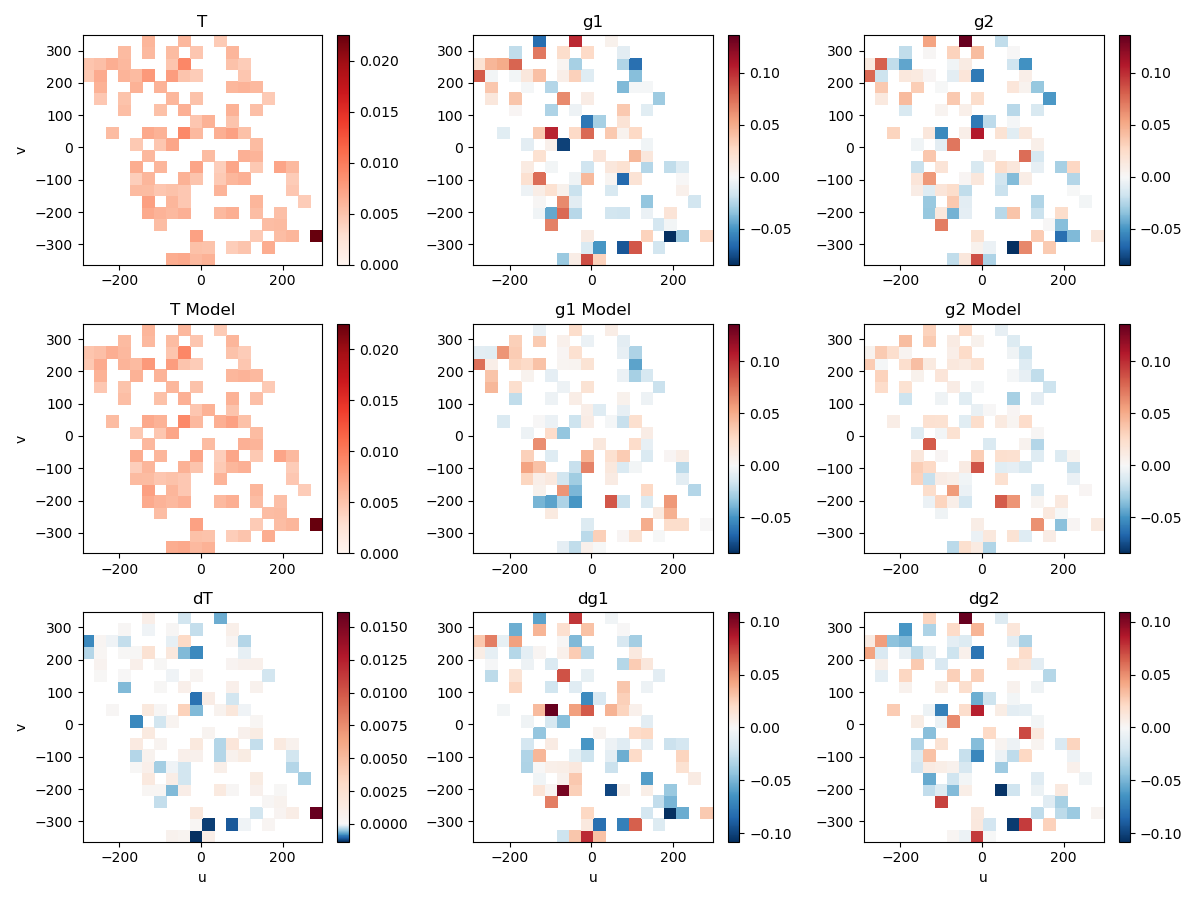
\includegraphics[width=.3\linewidth]{227wMedium/piff_twod.png}\hfill
  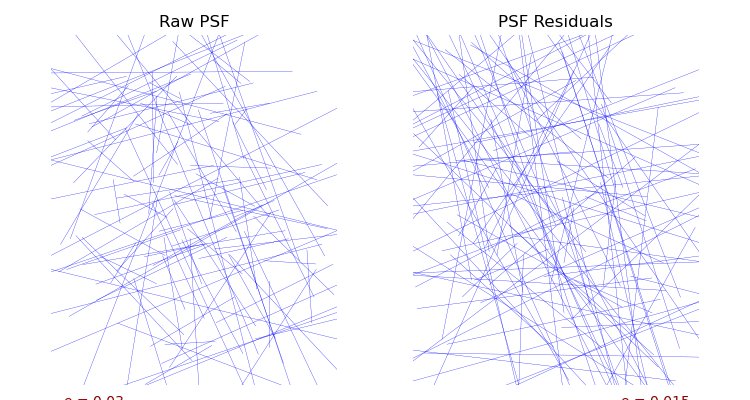
\includegraphics[width=.3\linewidth]{227wMedium/piff_whisker.png}\hfill
  \caption{f227w Medium}
  \end{subfigure}\par\medskip


\end{figure} \newpage
\begin{python}
# How large should the postage stamp cutouts of the stars be?
    stamp_size: 30

model:
    # This model uses a grid of pixels to model the surface brightness distribution.
    type: PixelGrid
    scale: 0.040      # NIRCam ative pixel scale
    size: 30          # Model is 24 x 24 in these
\end{python}\\
\begin{figure}[!h]
  \begin{subfigure}{\linewidth}
  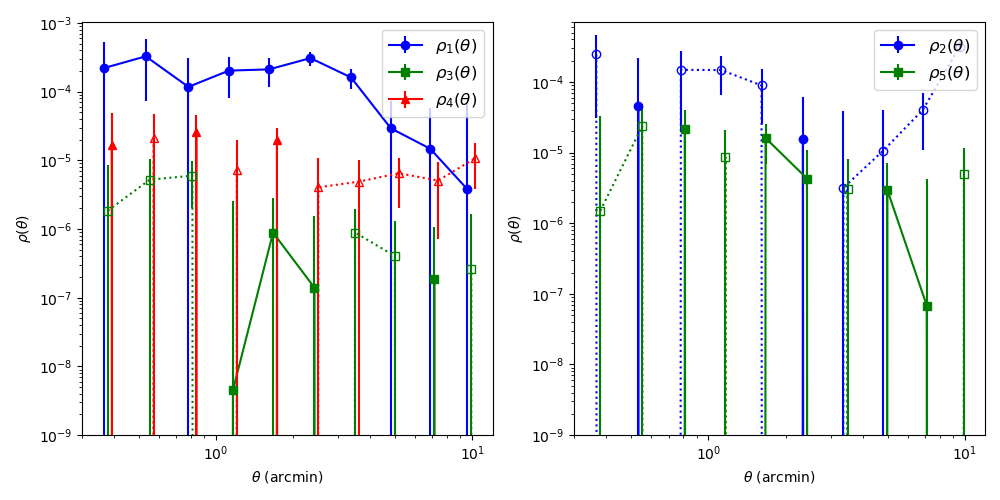
\includegraphics[width=.3\linewidth]{227wCoarse/piff_rho.png}\hfill
  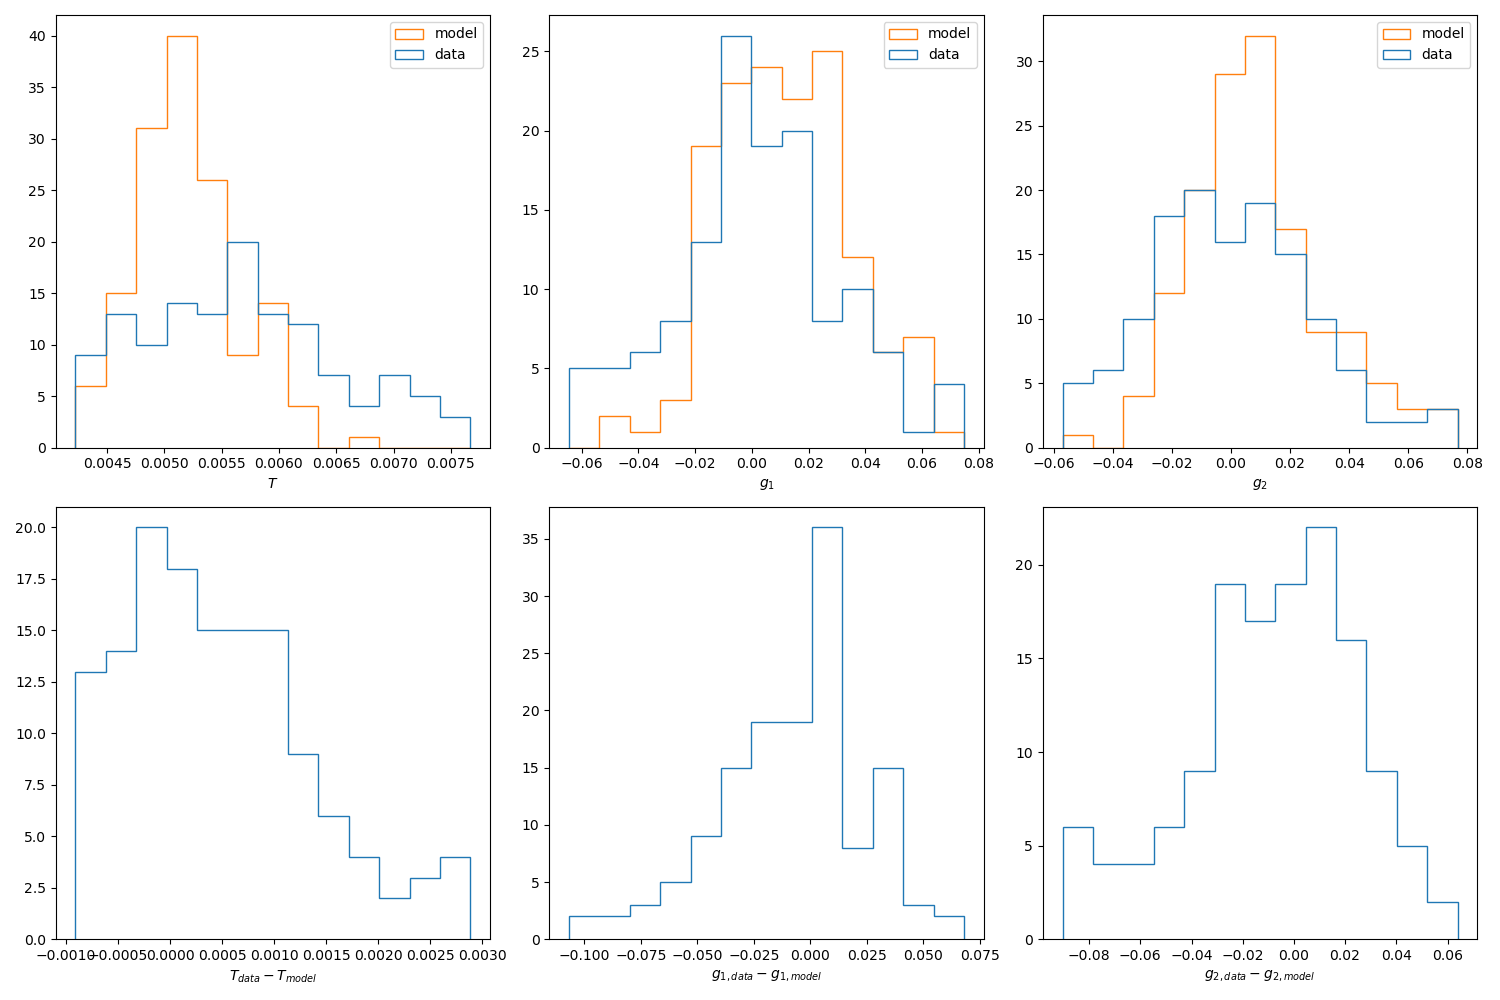
\includegraphics[width=.3\linewidth]{227wCoarse/piff_shapes.png}\hfill
  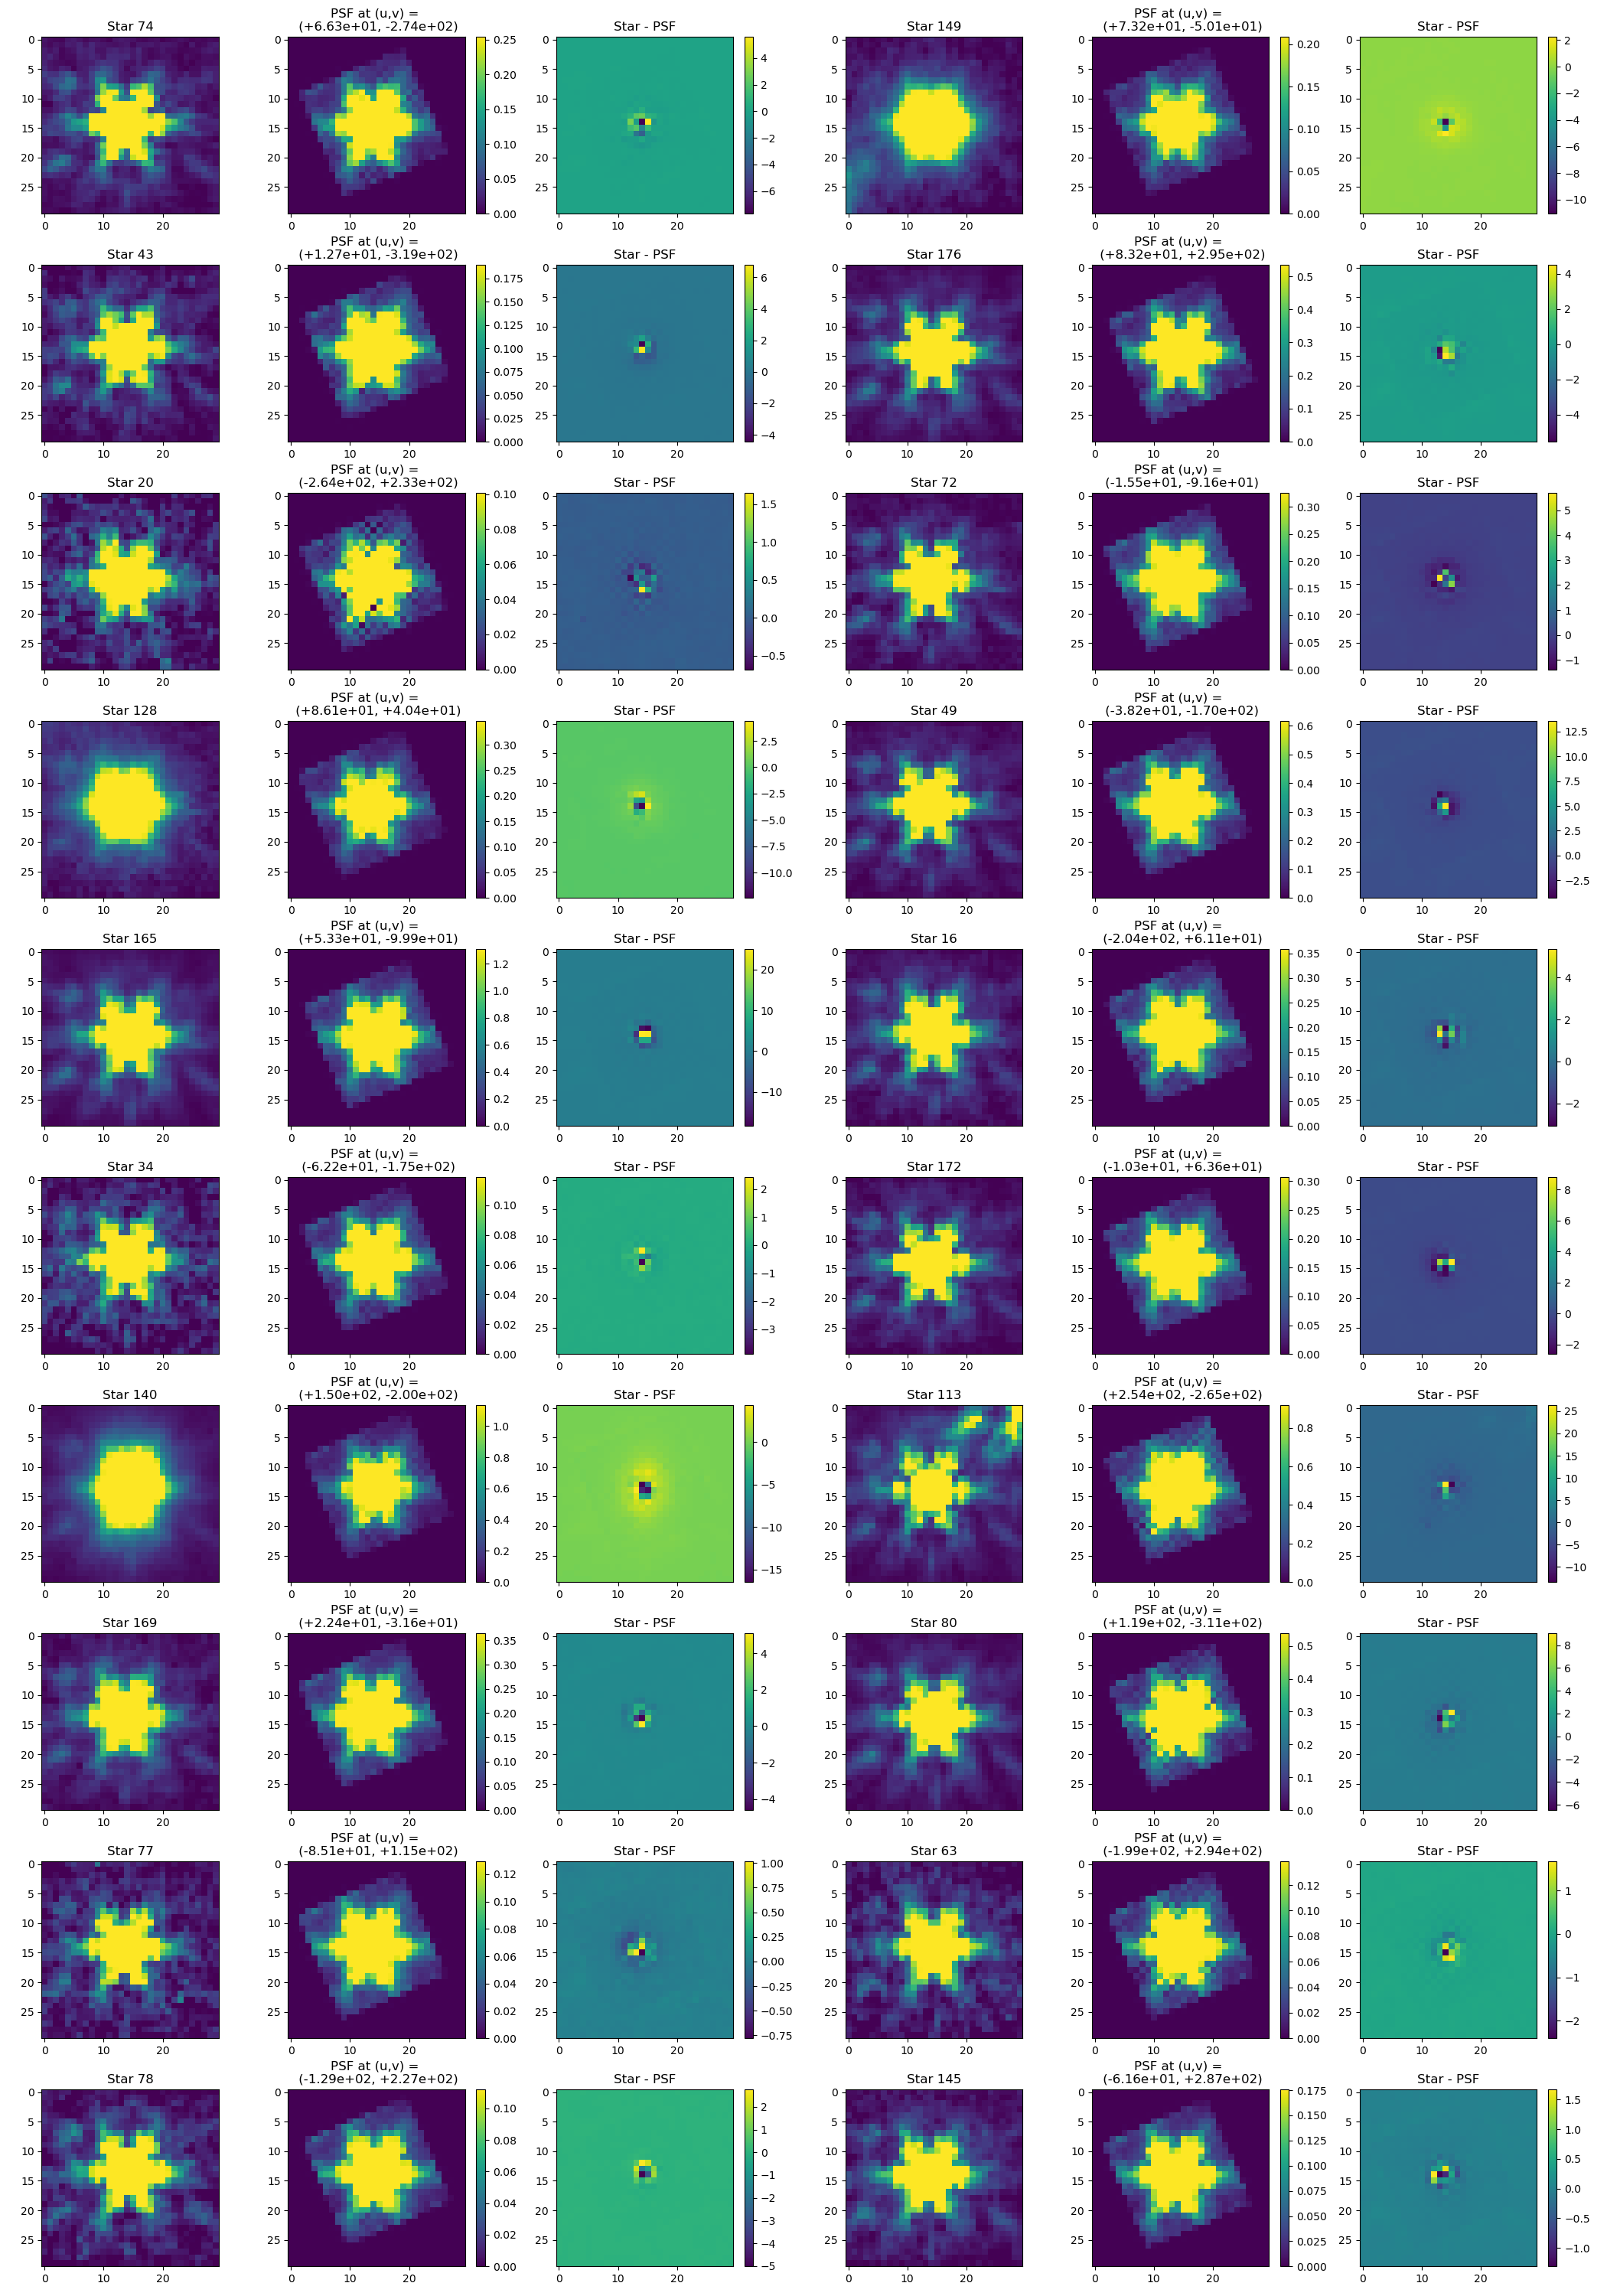
\includegraphics[width=.3\linewidth]{227wCoarse/piff_stars.png}
  \end{subfigure}\par\medskip
  \begin{subfigure}{\linewidth}
  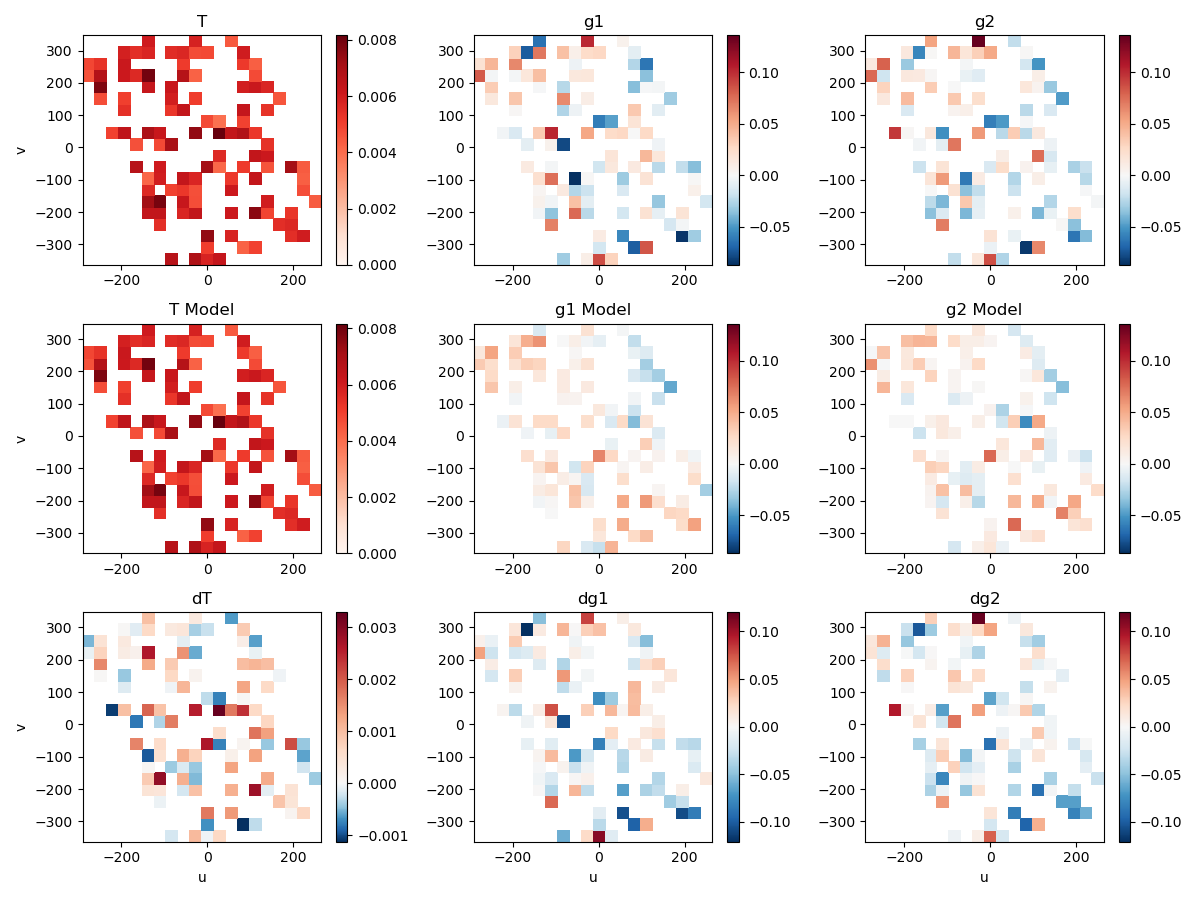
\includegraphics[width=.3\linewidth]{227wCoarse/piff_twod.png}\hfill
  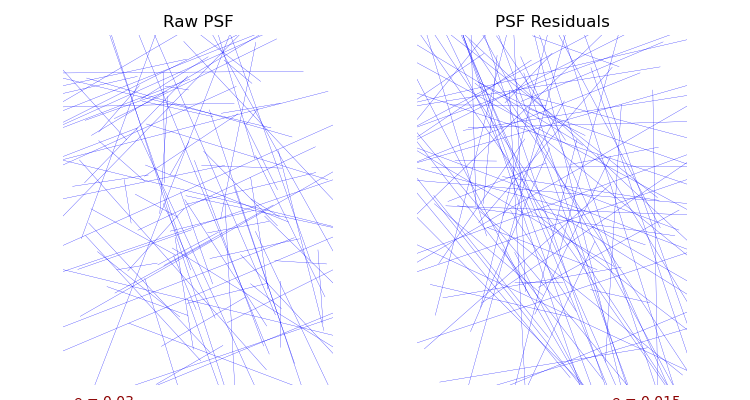
\includegraphics[width=.3\linewidth]{227wCoarse/piff_whisker.png}\hfill
  \caption{f227w Coarse}
  \end{subfigure}\par\medskip


\end{figure} \newpage

\newpage
\section{Ill-conditioned matrices}
\noindent {\begin{tikzpicture}[outline/.style={draw=#1,thick,fill=#1!50}]
\node [outline=red] at (0,1) {\bf ill-conditioned matrices};
\end{tikzpicture}}\\
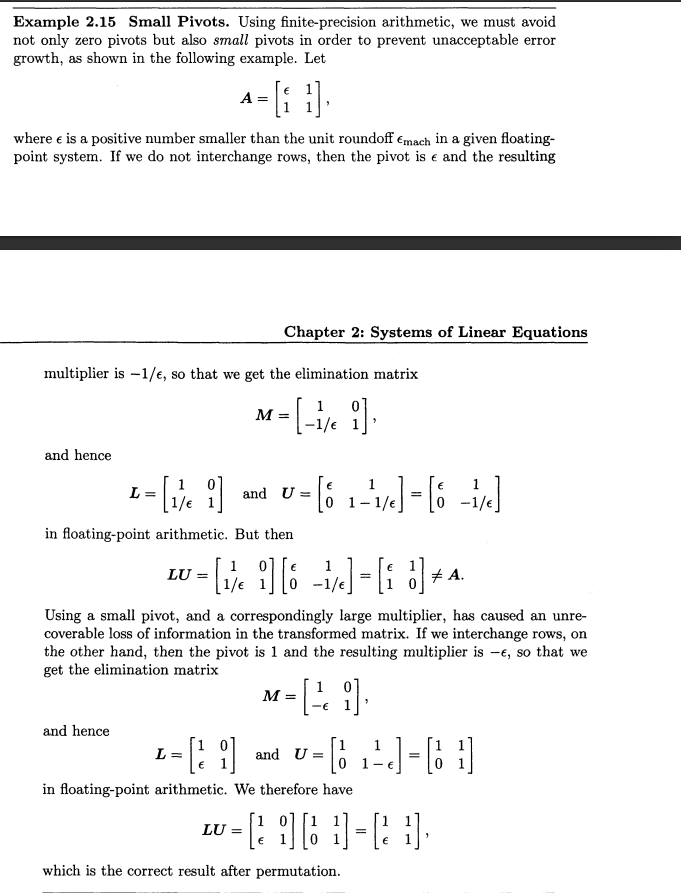
\includegraphics[scale=0.4]{Screenshot from 2023-02-13 12-08-58.png}
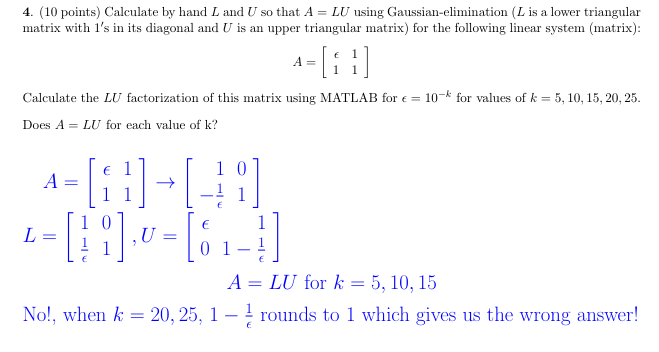
\includegraphics[scale=0.4]{Screenshot from 2023-02-13 12-11-33.png}\\
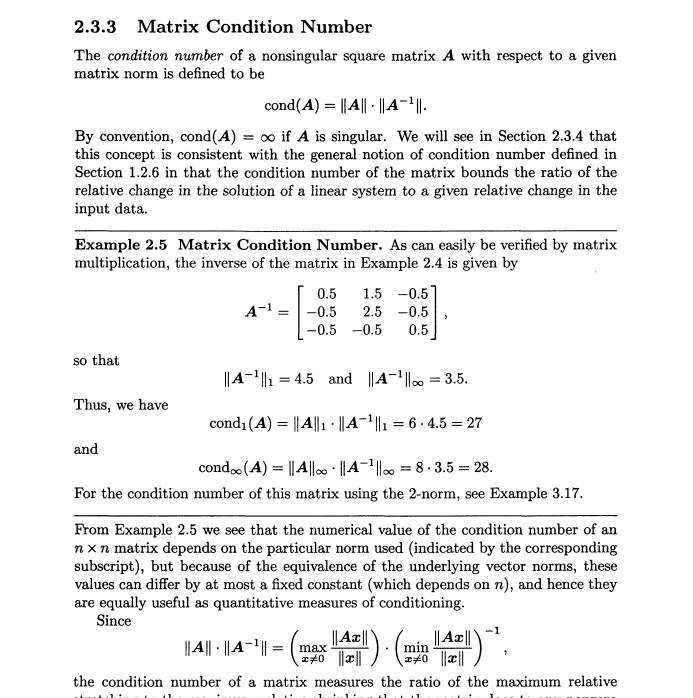
\includegraphics[scale=0.4]{Screenshot from 2023-02-13 12-16-08.png}
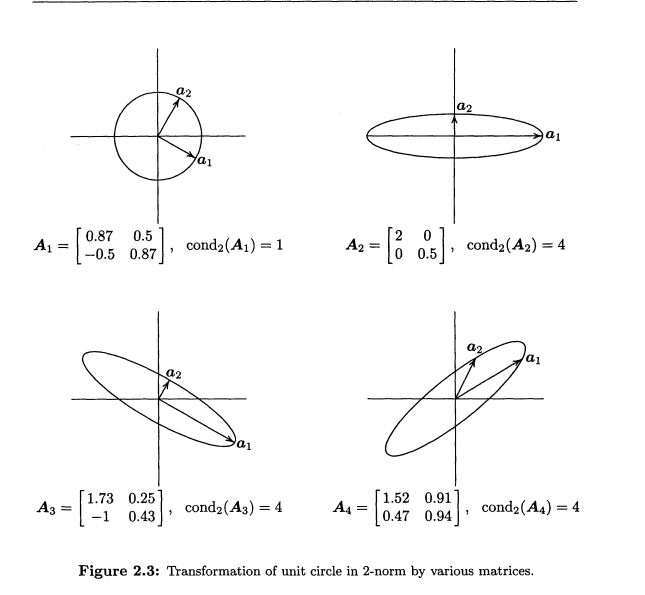
\includegraphics[scale=0.4]{Screenshot from 2023-02-13 12-17-24.png}\\
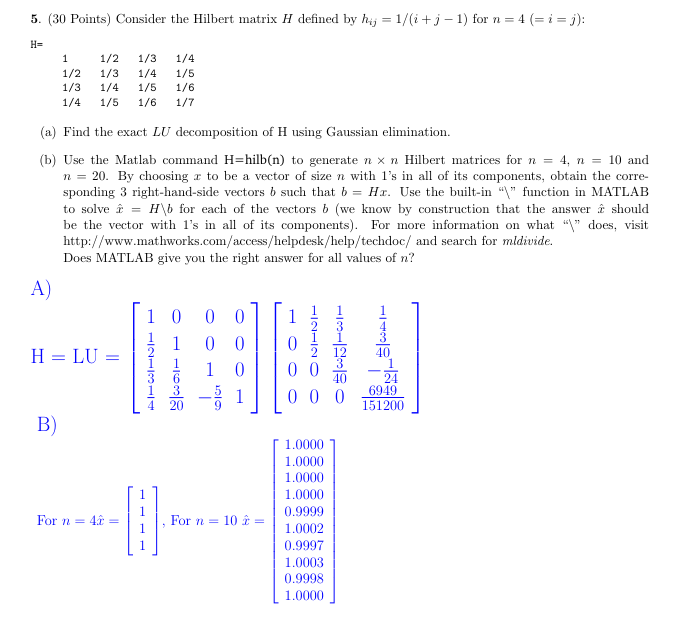
\includegraphics[scale=0.4]{Screenshot from 2023-02-13 12-24-42.png}
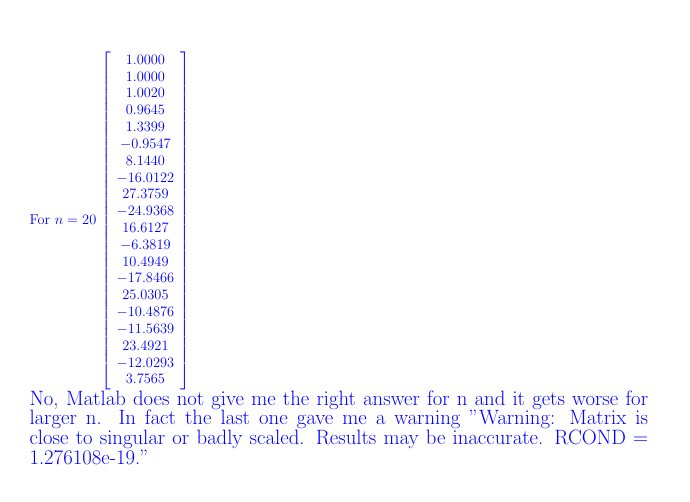
\includegraphics[scale=0.4]{Screenshot from 2023-02-13 12-24-50.png}

\newpage
\section{Application Materials}
\noindent {\begin{tikzpicture}[outline/.style={draw=#1,thick,fill=#1!50}]
\node [outline=red] at (0,1) {\bf application materials};
\end{tikzpicture}}\\
\begin{enumerate}
    \item First application is basically done
    \item Second is confusing because they don't ask for a resume, should I include my accomplishments in the two page research proposal. What are some things I can add to my research proposal to increase my chances of getting it accepted
    \item Made a resume version of CV, for the sake of abiding by their rules
\end{enumerate}
\section{Lingering questions}
\begin{enumerate}
    \item Where do these parameters come from. Some material from my courses are starting to give me more machinery to think about how PIFF is working under the hood and I'd like to know how I may go about choosing the parameters I attempt to estimate
\end{enumerate}
\section{To-do}
\begin{enumerate}
    \item Be more efficient in running getpsf
    \item Submit apps
    \item $\left[\text{What we come up with during meeting}\right]$
\end{enumerate}

\end{document}
%%------------ Arman Shokrollahi--------------%%
